\documentclass{article}
\usepackage{amsmath}
\usepackage{fullpage}
\usepackage{multicol}
%\usepackage{graphicx}
\usepackage{tikz}
\usetikzlibrary{calc}
% \usepackage{pgfmath}
\usepackage[aux]{rerunfilecheck}

% Macros for MATH 110 course dates

\newcommand{\commonTheme}{metropolis}
\newcommand{\commonColorTheme}{metropolis}

\newcommand{\commonAuthor}{Edward Doolittle}
\newcommand{\commonInstitute}{Department of Indigenous Knowledge and
  Science \\ First Nations University of Canada}
\newcommand{\commonCourse}{MATH 110 Calculus I}
\newcommand{\commonTerm}{202510}
\newcommand{\commonDate}{January 6, 2025}

% Review Material

% Lab 0
\newcommand{\commonEventNegativeOne}{LabNegativeOne}
\newcommand{\commonDateLabNegativeOne}{Monday, January 6, 2025}
\newcommand{\commonTitleLabNegativeOne}{MATH 110 Lab 0}
\newcommand{\commonSubtitleLabNegativeOne}{No Lab; Course Opens}

% Section 001
\newcommand{\commonEventZeroZeroOne}{ZeroZeroOne}
\newcommand{\commonDateZeroZeroOne}{Tuesday, January 7, 2025}
\newcommand{\commonTitleZeroZeroOne}{MATH 110 Review 0.1}
\newcommand{\commonSubtitleZeroZeroOne}{Review of Algebra}
\newcommand{\commonPSTitleZeroZeroOne}{MATH 110 Review Problem Set 0.1}

% Section 00A
\newcommand{\commonEventZeroZeroA}{ZeroZeroA}
\newcommand{\commonDateZeroZeroA}{Tuesday, January 7, 2025}
\newcommand{\commonTitleZeroZeroA}{MATH 110 Review 0.A}
\newcommand{\commonSubtitleZeroZeroA}{Review of Inequalities and
  Absolute Values}
\newcommand{\commonPSTitleZeroZeroA}{MATH 110 Review Problem Set 0.A}

% Section 00B
\newcommand{\commonEventZeroZeroB}{ZeroZeroB}
\newcommand{\commonDateZeroZeroB}{Tuesday, January 7, 2025}
\newcommand{\commonTitleZeroZeroB}{MATH 110 Review 0.B}
\newcommand{\commonSubtitleZeroZeroB}{Review of Coordinate Geometry
  and Lines}
\newcommand{\commonPSTitleZeroZeroB}{MATH 110 Review Problem Set 0.B}

% Section 00C
\newcommand{\commonEventZeroZeroC}{ZeroZeroC}
\newcommand{\commonDateZeroZeroC}{Thursday, January 9, 2025}
\newcommand{\commonTitleZeroZeroC}{MATH 110 Review 0.C}
\newcommand{\commonSubtitleZeroZeroC}{Review of Graphs of Second
  Degree Equations}
\newcommand{\commonPSTitleZeroZeroC}{MATH 110 Review Problem Set 0.C}

% Section 00D
\newcommand{\commonEventZeroZeroD}{ZeroZeroD}
\newcommand{\commonDateZeroZeroD}{Thursday, January 9, 2025}
\newcommand{\commonTitleZeroZeroD}{MATH 110 Review 0.D}
\newcommand{\commonSubtitleZeroZeroD}{Review of Trigonometry}
\newcommand{\commonPSTitleZeroZeroD}{MATH 110 Review Problem Set 0.D}

% Section 011
\newcommand{\commonEventZeroOneOne}{ZeroOneOne}
\newcommand{\commonDateZeroOneOne}{Thursday, January 9, 2025}
\newcommand{\commonTitleZeroOneOne}{MATH 110 Review 1.1}
\newcommand{\commonSubtitleZeroOneOne}{Review of Functions}
\newcommand{\commonPSTitleZeroOneOne}{MATH 110 Review Problem Set 1.1}


% Main Course

% Lab 1
\newcommand{\commonEventZero}{LabZero}
\newcommand{\commonDateLabZero}{Monday, January 13, 2025}
\newcommand{\commonTitleLabZero}{MATH 110 Lab 1}
\newcommand{\commonSubtitleLabZero}{Quiz 0: STACK, Onboarding}

% Section 1.4
\newcommand{\commonEventOne}{ZeroOneFour}
\newcommand{\commonDateZeroOneFour}{Tuesday, January 14, 2025}
\newcommand{\commonTitleZeroOneFour}{MATH 110 Lecture 1.4}
\newcommand{\commonSubtitleZeroOneFour}{The Tangent and Velocity Problems}
\newcommand{\commonPSTitleZeroOneFour}{MATH 110 Problem Set 1.4}

% Section 1.5
\newcommand{\commonEventTwo}{ZeroOneFive}
\newcommand{\commonDateZeroOneFive}{Thursday, January 16, 2025}
\newcommand{\commonTitleZeroOneFive}{MATH 110 Lecture 1.5}
\newcommand{\commonSubtitleZeroOneFive}{The Limit of a Function}
\newcommand{\commonPSTitleZeroOneFive}{MATH 110 Problem Set 1.5}

% Lab 2
\newcommand{\commonEventThree}{LabOne}
\newcommand{\commonDateLabOne}{Monday, January 20, 2025}
\newcommand{\commonTitleLabOne}{MATH 110 Lab 2}
\newcommand{\commonSubtitleLabOne}{Quiz 1: Review}

% Section 1.6
\newcommand{\commonEventFour}{ZeroOneSix}
\newcommand{\commonDateZeroOneSix}{Tuesday, January 21, 2025}
\newcommand{\commonTitleZeroOneSix}{MATH 110 Lecture 1.6}
\newcommand{\commonSubtitleZeroOneSix}{Calculating Limits Using the Limit Laws}
\newcommand{\commonPSTitleZeroOneSix}{MATH 110 Problem Set 1.6}

% Section 1.7
\newcommand{\commonEventFive}{ZeroOneSeven}
\newcommand{\commonDateZeroOneSeven}{(Not covered)}
\newcommand{\commonTitleZeroOneSeven}{MATH 110 Lecture 1.7}
\newcommand{\commonSubtitleZeroOneSeven}{The Precise Definition of a Limit}
\newcommand{\commonPSTitleZeroOneSeven}{MATH 110 Problem Set 1.7}

% Section 1.8
\newcommand{\commonEventSix}{ZeroOneEight}
\newcommand{\commonDateZeroOneEight}{Thursday, January 23, 2025}
\newcommand{\commonTitleZeroOneEight}{MATH 110 Lecture 1.8}
\newcommand{\commonSubtitleZeroOneEight}{Continuity}
\newcommand{\commonPSTitleZeroOneEight}{MATH 110 Problem Set 1.8}

% Lab 3
\newcommand{\commonEventSeven}{LabTwo}
\newcommand{\commonDateLabTwo}{Monday, January 27, 2025}
\newcommand{\commonTitleLabTwo}{MATH 110 Lab 3}
\newcommand{\commonSubtitleLabTwo}{Quiz 2: Sections 1.4, 1.5}

% Section 2.1
\newcommand{\commonEventEight}{ZeroTwoOne}
\newcommand{\commonDateZeroTwoOne}{Tuesday, January 28, 2025}
\newcommand{\commonTitleZeroTwoOne}{MATH 110 Lecture 2.1}
\newcommand{\commonSubtitleZeroTwoOne}{Derivatives and Rates of Change}
\newcommand{\commonPSTitleZeroTwoOne}{MATH 110 Problem Set 2.1}

% Section 2.2
\newcommand{\commonEventNine}{ZeroTwoTwo}
\newcommand{\commonDateZeroTwoTwo}{Thursday, January 30, 2025}
\newcommand{\commonTitleZeroTwoTwo}{MATH 110 Lecture 2.2}
\newcommand{\commonSubtitleZeroTwoTwo}{The Derivative as a Function}
\newcommand{\commonPSTitleZeroTwoTwo}{MATH 110 Problem Set 2.2}

% Lab 4
\newcommand{\commonEventTen}{LabThree}
\newcommand{\commonDateMTOne}{Monday, February 3, 2025} 
\newcommand{\commonDateLabThree}{Monday, February 3, 2025}
\newcommand{\commonTitleLabThree}{MATH 110 Lab 4}
\newcommand{\commonSubtitleLabThree}{Midterm: Review, Chapter 1}

% Section 2.3
\newcommand{\commonEventEleven}{ZeroTwoThree}
\newcommand{\commonDateZeroTwoThree}{Tuesday, February 4, 2025}
\newcommand{\commonTitleZeroTwoThree}{MATH 110 Lecture 2.3}
\newcommand{\commonSubtitleZeroTwoThree}{Differentiation Formulas}
\newcommand{\commonPSTitleZeroTwoThree}{MATH 110 Problem Set 2.3}

% Section 2.4
\newcommand{\commonEventTwelve}{ZeroTwoFour}
\newcommand{\commonDateZeroTwoFour}{Thursday, February 6, 2025}
\newcommand{\commonTitleZeroTwoFour}{MATH 110 Lecture 2.4}
\newcommand{\commonSubtitleZeroTwoFour}{Derivatives of Trigonometric Functions}
\newcommand{\commonPSTitleZeroTwoFour}{MATH 110 Problem Set 2.4}

% Lab 5
\newcommand{\commonEventThirteen}{LabFour}
\newcommand{\commonDateLabFour}{Monday, February 10, 2025}
\newcommand{\commonTitleLabFour}{MATH 110 Lab 5}
\newcommand{\commonSubtitleLabFour}{Quiz 3: Sections 2.1, 2.2}

% Section 2.5
\newcommand{\commonEventFourteen}{ZeroTwoFive}
\newcommand{\commonDateZeroTwoFive}{Tuesday, February 11, 2025}
\newcommand{\commonTitleZeroTwoFive}{MATH 110 Lecture 2.5}
\newcommand{\commonSubtitleZeroTwoFive}{The Chain Rule}
\newcommand{\commonPSTitleZeroTwoFive}{MATH 110 Problem Set 2.5}

% Section 2.6
\newcommand{\commonEventFifteen}{ZeroTwoSix}
\newcommand{\commonDateZeroTwoSix}{Thursday, February 13, 2025}
\newcommand{\commonTitleZeroTwoSix}{MATH 110 Lecture 2.6}
\newcommand{\commonSubtitleZeroTwoSix}{Implicit Differentiation}
\newcommand{\commonPSTitleZeroTwoSix}{MATH 110 Problem Set 2.6}

% Lab 6
\newcommand{\commonEventSixteen}{LabFive}
\newcommand{\commonDateLabFive}{Monday, February 24, 2025}
\newcommand{\commonTitleLabFive}{MATH 110 Lab 6}
\newcommand{\commonSubtitleLabFive}{Quiz 4: Sections 2.3, 2.4}

% Section 2.7
\newcommand{\commonEventSeventeen}{ZeroTwoSeven}
\newcommand{\commonDateZeroTwoSeven}{Tuesday, February 25, 2025}
\newcommand{\commonTitleZeroTwoSeven}{MATH 110 Lecture 2.7}
\newcommand{\commonSubtitleZeroTwoSeven}{Rates of Change in the
  Natural and Social Sciences}
\newcommand{\commonPSTitleZeroTwoSeven}{MATH 110 Problem Set 2.7}

% Section 2.8
\newcommand{\commonEventEighteen}{ZeroTwoEight}
\newcommand{\commonDateZeroTwoEight}{Thursday, February 27, 2025}
\newcommand{\commonTitleZeroTwoEight}{MATH 110 Lecture 2.8}
\newcommand{\commonSubtitleZeroTwoEight}{Related Rates}
\newcommand{\commonPSTitleZeroTwoEight}{MATH 110 Problem Set 2.8}

% Lab 7
\newcommand{\commonEventNineteen}{LabSix}
\newcommand{\commonDateLabSix}{Monday, March 3, 2025}
\newcommand{\commonTitleLabSix}{MATH 110 Lab 7}
\newcommand{\commonSubtitleLabSix}{Quiz 5: Sections 2.5, 2.6}

% Section 3.1
\newcommand{\commonEventTwenty}{ZeroThreeOne}
\newcommand{\commonDateZeroThreeOne}{Tuesday, March 4, 2025}
\newcommand{\commonTitleZeroThreeOne}{MATH 110 Lecture 3.1}
\newcommand{\commonSubtitleZeroThreeOne}{Maximum and Minimum Values}
\newcommand{\commonPSTitleZeroThreeOne}{MATH 11 Problem Set 3.1}

% Section 3.2
\newcommand{\commonEventTwentyOne}{ZeroThreeTwo}
\newcommand{\commonDateZeroThreeTwo}{Thursday, March 6, 2025}
\newcommand{\commonTitleZeroThreeTwo}{MATH 110 Lecture 3.2}
\newcommand{\commonSubtitleZeroThreeTwo}{The Mean Value Theorem}
\newcommand{\commonPSTitleZeroThreeTwo}{MATH 110 Problem Set 3.2}

% Lab 8
\newcommand{\commonEventTwentyTwo}{LabSeven}
\newcommand{\commonDateMTTwo}{Monday, March 10, 2025}
\newcommand{\commonDateLabSeven}{Monday, March 10, 2025}
\newcommand{\commonTitleLabSeven}{MATH 110 Lab 8}
\newcommand{\commonSubtitleLabSeven}{Midterm: Chapter 2}

% Section 3.3
\newcommand{\commonEventTwentyThree}{ZeroThreeThree}
\newcommand{\commonDateZeroThreeThree}{Tuesday, March 11, 2025}
\newcommand{\commonTitleZeroThreeThree}{MATH 110 Lecture 3.3}
\newcommand{\commonSubtitleZeroThreeThree}{How Derivatives Affect the
  Shape of a Graph}
\newcommand{\commonPSTitleZeroThreeThree}{MATH 110 Problem Set 3.3}

% Section 3.4
\newcommand{\commonEventTwentyFour}{ZeroThreeFour}
\newcommand{\commonDateZeroThreeFour}{Thursday, March 13, 2025}
\newcommand{\commonTitleZeroThreeFour}{MATH 110 Lecture 3.4}
\newcommand{\commonSubtitleZeroThreeFour}{Limits at Infinity;
  Horizontal Asymptotes}
\newcommand{\commonPSTitleZeroThreeFour}{MATH 110 Problem Set 3.4}

% Lab 9
\newcommand{\commonEventTwentyFive}{LabEight}
\newcommand{\commonDateLabEight}{Monday, March 17, 2025}
\newcommand{\commonTitleLabEight}{MATH 110 Lab 9}
\newcommand{\commonSubtitleLabEight}{Quiz 6: Sections 3.1, 3.2}

% Section 3.5
\newcommand{\commonEventTwentySix}{ZeroThreeFive}
\newcommand{\commonDateZeroThreeFive}{Tuesday, March 18, 2025}
\newcommand{\commonTitleZeroThreeFive}{MATH 110 Lecture 3.5}
\newcommand{\commonSubtitleZeroThreeFive}{Summary of Curve Sketching}
\newcommand{\commonPSTitleZeroThreeFive}{MATH 110 Problem Set 3.5}

% Section 3.7
\newcommand{\commonEventTwentySeven}{ZeroThreeSeven}
\newcommand{\commonDateZeroThreeSeven}{Thursday, March 20, 2025}
\newcommand{\commonTitleZeroThreeSeven}{MATH 110 Lecture 3.7}
\newcommand{\commonSubtitleZeroThreeSeven}{Optimization Problems}
\newcommand{\commonPSTitleZeroThreeSeven}{MATH 110 Problem Set 3.7}

% Lab 10
\newcommand{\commonEventTwentyEight}{LabNine}
\newcommand{\commonDateLabNine}{Monday, March 24, 2025}
\newcommand{\commonTitleLabNine}{MATH 110 Lab 10}
\newcommand{\commonSubtitleLabNine}{Quiz 7: Sections 3.3, 3.4}

% Section 4.1
\newcommand{\commonEventTwentyNine}{ZeroFourOne}
\newcommand{\commonDateZeroFourOne}{Tuesday, March 25, 2025}
\newcommand{\commonTitleZeroFourOne}{MATH 110 Lecture 4.1}
\newcommand{\commonSubtitleZeroFourOne}{Areas and Distances}
\newcommand{\commonPSTitleZeroFourOne}{MATH 110 Problem Set 4.1}

% Section 4.2
\newcommand{\commonEventThirty}{ZeroFourTwo}
\newcommand{\commonDateZeroFourTwo}{Thursday, March 27, 2025}
\newcommand{\commonTitleZeroFourTwo}{MATH 110 Lecture 4.2}
\newcommand{\commonSubtitleZeroFourTwo}{The Definite Integral}
\newcommand{\commonPSTitleZeroFourTwo}{MATH 110 Problem Set 4.2}

% Lab 11
\newcommand{\commonEventThirtyOne}{LabTen}
\newcommand{\commonDateLabTen}{Monday, March 31, 2025}
\newcommand{\commonTitleLabTen}{MATH 110 Lab 11}
\newcommand{\commonSubtitleLabTen}{Quiz 8: Sections 3.5, 3.7}

% Section 4.3
\newcommand{\commonEventThirtyTwo}{ZeroFourThree}
\newcommand{\commonDateZeroFourThree}{Tuesday, April 1, 2025}
\newcommand{\commonTitleZeroFourThree}{MATH 110 Lecture 4.3}
\newcommand{\commonSubtitleZeroFourThree}{The Fundamental Theorem of Calculus}
\newcommand{\commonPSTitleZeroFourThree}{MATH 110 Problem Set 4.3}

% Section 4.4
\newcommand{\commonEventThirtyThree}{ZeroFourFour}
\newcommand{\commonDateZeroFourFour}{Thursday, April 3, 2025}
\newcommand{\commonTitleZeroFourFour}{MATH 110 Lecture 4.4}
\newcommand{\commonSubtitleZeroFourFour}{Indefinite Integrals and the
  Net Change Theorem}
\newcommand{\commonPSTitleZeroFourFour}{MATH 110 Problem Set 4.4}

% Lab 12
\newcommand{\commonEventThirtyFour}{LabEleven}
\newcommand{\commonDateLabEleven}{Monday, April 7, 2025}
\newcommand{\commonTitleLabEleven}{MATH 110 Lab 12}
\newcommand{\commonSubtitleLabEleven}{Quiz 9: Sections 4.1, 4.2}

% Section 4.5
\newcommand{\commonEventThirtyFive}{ZeroFourFive}
\newcommand{\commonDateZeroFourFive}{Tuesday, April 8, 2025}
\newcommand{\commonTitleZeroFourFive}{MATH 110 Lecture 4.5}
\newcommand{\commonSubtitleZeroFourFive}{The Substitution Rule}
\newcommand{\commonPSTitleZeroFourFive}{MATH 110 Problem Set 4.5}

% Section 5.1
\newcommand{\commonEventThirtySix}{ZeroFiveOne}
\newcommand{\commonDateZeroFiveOne}{Thursday, April 10, 2025}
\newcommand{\commonTitleZeroFiveOne}{MATH 110 Lecture 5.1}
\newcommand{\commonSubtitleZeroFiveOne}{Areas Between Curves}
\newcommand{\commonPSTitleZeroFiveOne}{MATH 110 Problem Set 5.1}

% Lab 13
\newcommand{\commonEventThirtySeven}{LabTwelve}
\newcommand{\commonDateLabTwelve}{Monday, April 14, 2025}
\newcommand{\commonTitleLabTwelve}{MATH 110 Review Lab}
\newcommand{\commonSubtitleLabTwelve}{Bonus Quiz 10: Sections 4.3, 4.4}

% Final Class
\newcommand{\commonEventThirtyEight}{FinalClass}
\newcommand{\commonDateFinalClass}{Tuesday, April 15, 2025}
\newcommand{\commonTitleFinalClass}{MATH 110 Review Class}
\newcommand{\commonSubtitleFinalClass}{Answer Questions, Review for Exam}

% Final Exam
\newcommand{\commonEventThirtyNine}{Final}
\newcommand{\commonDateFinal}{Thursday, April 22, 2025}
\newcommand{\commonTitleFinal}{MATH 110 Final Exam}
\newcommand{\commonSubtitleFinal}{Comprehensive Exam: All Sections}

% Orphaned -- no longer part of the course

% Section 2.9
\newcommand{\commonDateZeroTwoNine}{Not part of the course}
\newcommand{\commonTitleZeroTwoNine}{MATH 110 Lecture 2.9}
\newcommand{\commonSubtitleZeroTwoNine}{Linear Approximations and Differentials}
\newcommand{\commonPSTitleZeroTwoNine}{MATH 110 Problem Set 2.9}


% % Introduction
% \newcommand{\commonEventOneDate}{Wednesday, September 8, 2010}
% \newcommand{\commonEventOneDesc}{Introduction to the Course}
% \newcommand{\commonDateZeroZeroZero}{September 8, 2010}
% \newcommand{\commonTitleZeroZeroZero}{MATH 104 Introduction}
% \newcommand{\commonSubtitleZeroZeroZero}{Outline of the Course}

% % Lecture 1
% \newcommand{\commonEventTwoDate}{Friday, September 10, 2010}
% \newcommand{\commonEventTwoDesc}{Lecture 1: Algebra}
% \newcommand{\commonDateZeroZeroOne}{September 10, 2010}
% \newcommand{\commonTitleZeroZeroOne}{MATH 104 Lecture 1}
% \newcommand{\commonSubtitleZeroZeroOne}{Review of Algebra}
% % associated evaluation ... factor this out?
% \newcommand{\commonPSTitleZeroZeroOne}{MATH 104 Problem Set 1}
% \newcommand{\commonEvalZeroZeroOne}{Quiz 1}
% \newcommand{\commonEvalDateZeroZeroOne}{Wednesday, September 15, 2010}

% % Lecture 2
% \newcommand{\commonEventThreeDate}{Monday, September 13, 2010}
% \newcommand{\commonEventThreeDesc}{Lecture 2: Appendix A}
% \newcommand{\commonDateZeroZeroA}{September 13, 2010}
% \newcommand{\commonTitleZeroZeroA}{MATH 104 Lecture 2}
% \newcommand{\commonSubtitleZeroZeroA}{Appendix A: Numbers, Inequalities, 
%   and Absolute Values}
% % associated evaluation ... factor this out?
% \newcommand{\commonPSTitleZeroZeroA}{MATH 104 Problem Set 2}
% \newcommand{\commonEvalZeroZeroA}{Quiz 2}
% \newcommand{\commonEvalDateZeroZeroA}{Wednesday, September 22, 2010}

% % Review 1
% \newcommand{\commonEventFourDate}{Wednesday, September 15, 2010}
% \newcommand{\commonEventFourDesc}{Review 1: Review Algebra; Quiz 1; Review Appendix A}
% \newcommand{\commonDateRZeroOne}{September 15, 2010}
% \newcommand{\commonTitleRZeroOne}{MATH 104 Review 1}
% \newcommand{\commonSubtitleRZeroOne}{Review of Algebra, Appendix A}

% % Lecture 3
% \newcommand{\commonEventFiveDate}{Friday, September 17, 2010}
% \newcommand{\commonEventFiveDesc}{Lecture 3: Appendix B}
% \newcommand{\commonDateZeroZeroB}{September 17, 2010}
% \newcommand{\commonTitleZeroZeroB}{MATH 104 Lecture 3}
% \newcommand{\commonSubtitleZeroZeroB}{Appendix B: Coordinate Geometry and Lines}
% % associated evaluation ... factor this out?
% \newcommand{\commonPSTitleZeroZeroB}{MATH 104 Problem Set 3}
% \newcommand{\commonEvalZeroZeroB}{Quiz 2}
% \newcommand{\commonEvalDateZeroZeroB}{Wednesday, September 22, 2010}

% % Lecture 4
% \newcommand{\commonEventSixDate}{Monday, Sepbember 20, 2010}
% \newcommand{\commonEventSixDesc}{Lecture 4: Appendix C}
% \newcommand{\commonDateZeroZeroC}{September 20, 2010}
% \newcommand{\commonTitleZeroZeroC}{MATH 104 Lecture 4}
% \newcommand{\commonSubtitleZeroZeroC}{Appendix C: Graphs of Second-Degree Equations}
% % associated evaluation ... factor this out?
% \newcommand{\commonPSTitleZeroZeroC}{MATH 104 Problem Set 4}
% \newcommand{\commonEvalZeroZeroC}{Midterm 0}
% \newcommand{\commonEvalDateZeroZeroC}{Wednesday, September 29, 2010}

% % Review 2
% \newcommand{\commonEventSevenDate}{Wednesday, September 22, 2010}
% \newcommand{\commonEventSevenDesc}{Review 2: Review Appendix B; Quiz 2; Review Appendix C}
% \newcommand{\commonDateRZeroTwo}{September 22, 2010}
% \newcommand{\commonTitleRZeroTwo}{MATH 104 Review 2}
% \newcommand{\commonSubtitleRZeroTwo}{Review of Appendices B and C}

% % Lecture 5
% \newcommand{\commonEventEightDate}{Friday, September 24, 2010}
% \newcommand{\commonEventEightDesc}{Lecture 5: Appendix D}
% \newcommand{\commonDateZeroZeroD}{September 24, 2010}
% \newcommand{\commonTitleZeroZeroD}{MATH 104 Lecture 5}
% \newcommand{\commonSubtitleZeroZeroD}{Appendix D: Trigonometry}
% % associated evaluation ... factor this out?
% \newcommand{\commonPSTitleZeroZeroD}{MATH 104 Problem Set 5}
% \newcommand{\commonEvalZeroZeroD}{Midterm 0}
% \newcommand{\commonEvalDateZeroZeroD}{Wednesday, September 29, 2010}

% % Lecture 6
% \newcommand{\commonEventNineDate}{Monday, September 27, 2010}
% \newcommand{\commonEventNineDesc}{Lecture 6: Section 1.1}
% \newcommand{\commonDateZeroOneOne}{September 27, 2010}
% \newcommand{\commonTitleZeroOneOne}{MATH 104 Lecture 6}
% \newcommand{\commonSubtitleZeroOneOne}{Section 1.1: Four Ways to Represent a Function}
% % associated evaluation ... factor this out?
% \newcommand{\commonPSTitleZeroOneOne}{MATH 104 Problem Set 6}
% \newcommand{\commonEvalZeroOneOne}{Quiz 3}
% \newcommand{\commonEvalDateZeroOneOne}{Wednesday, October 6, 2010}

% % Review 3
% \newcommand{\commonEventTenDate}{Wednesday, September 29, 2010}
% \newcommand{\commonEventTenDesc}{Review 3: Review Appendix D; 
%   Self-Assessment Midterm 0}
% \newcommand{\commonDateRZeroThree}{September 29, 2010}
% \newcommand{\commonTitleRZeroThree}{MATH 104 Review 3}
% \newcommand{\commonSubtitleRZeroThree}{Review of Appendix D}

% % Lecture 7
% \newcommand{\commonEventElevenDate}{Friday, October 1, 2010}
% \newcommand{\commonEventElevenDesc}{Lecture 7: Section 1.2}
% \newcommand{\commonDateZeroOneTwo}{October 1, 2010}
% \newcommand{\commonTitleZeroOneTwo}{MATH 104 Lecture 7}
% \newcommand{\commonSubtitleZeroOneTwo}{Section 1.2: Mathematical Models: A Catalog of Essential Functions}
% % associated evaluation ... factor this out?
% \newcommand{\commonPSTitleZeroOneTwo}{MATH 104 Problem Set 7}
% \newcommand{\commonEvalZeroOneTwo}{Quiz 3}
% \newcommand{\commonEvalDateZeroOneTwo}{Wednesday, October 6, 2010}

% % Lecture 8
% \newcommand{\commonEventTwelveDate}{Monday, October 4, 2010}
% \newcommand{\commonEventTwelveDesc}{Lecture 8: Section 1.3}
% \newcommand{\commonDateZeroOneThree}{October 4, 2010}
% \newcommand{\commonTitleZeroOneThree}{MATH 104 Lecture 8}
% \newcommand{\commonSubtitleZeroOneThree}{Section 1.3: New Functions from Old Functions}
% % associated evaluation ... factor this out?
% \newcommand{\commonPSTitleZeroOneThree}{MATH 104 Problem Set 8}
% \newcommand{\commonEvalZeroOneThree}{Quiz 4}
% \newcommand{\commonEvalDateZeroOneThree}{Wednesday, October 13, 2010}

% % Review 4
% \newcommand{\commonEventThirteenDate}{Wednesday, October 6, 2010}
% \newcommand{\commonEventThirteenDesc}{Review 4: Review 1.1, 1.2; Quiz 3}
% \newcommand{\commonDateROneOne}{October 6, 2010}
% \newcommand{\commonTitleROneOne}{MATH 104 Review 4}
% \newcommand{\commonSubtitleROneOne}{Reveiw of 1.1, 1.2}

% % Lecture 9
% \newcommand{\commonEventFourteenDate}{Friday, October 8, 2010}
% \newcommand{\commonEventFourteenDesc}{Lecture 9: Section 1.4}
% \newcommand{\commonDateZeroOneFour}{October 8, 2010}
% \newcommand{\commonTitleZeroOneFour}{MATH 104 Lecture 9}
% \newcommand{\commonSubtitleZeroOneFour}{Section 1.4: Graphing Calculators and Computers}
% % associated evaluation ... factor this out?
% \newcommand{\commonPSTitleZeroOneFour}{MATH 104 Problem Set 9}
% \newcommand{\commonEvalZeroOneFour}{Quiz 4}
% \newcommand{\commonEvalDateZeroOneFour}{Wednesday, October 13, 2010}

% % Thanksgiving holiday
% \newcommand{\commonEventFifteenDate}{Monday, October 11, 2010}
% \newcommand{\commonEventFifteenDesc}{No class: Thanksgiving holiday}

% % Review 5
% \newcommand{\commonEventSixteenDate}{Wednesday, October 13, 2010}
% \newcommand{\commonEventSixteenDesc}{Review 5: Review 1.3, 1.4; Quiz 4}
% \newcommand{\commonDateROneTwo}{October 13, 2010}
% \newcommand{\commonTitleROneTwo}{MATH 104 Review 5}
% \newcommand{\commonSubtitleOneRTwo}{Review of 1.3, 1.4}

% % Lecture 10
% \newcommand{\commonEventSeventeenDate}{Friday, October 15, 2010}
% \newcommand{\commonEventSeventeenDesc}{Lecture 10: Section 1.5}
% \newcommand{\commonDateZeroOneFive}{October 15, 2010}
% \newcommand{\commonTitleZeroOneFive}{MATH 104 Lecture 10}
% \newcommand{\commonSubtitleZeroOneFive}{Section 1.5: Exponential Functions}
% % associated evaluation ... factor this out?
% \newcommand{\commonPSTitleZeroOneFive}{MATH 104 Problem Set 10}
% \newcommand{\commonEvalZeroOneFive}{Quiz 5}
% \newcommand{\commonEvalDateZeroOneFive}{Wednesday, October 20, 2010}

% % Lecture 11
% \newcommand{\commonEventEighteenDate}{Monday, October 18, 2010}
% \newcommand{\commonEventEighteenDesc}{Lecture 11: Section 1.6}
% \newcommand{\commonDateZeroOneSix}{October 18, 2010}
% \newcommand{\commonTitleZeroOneSix}{MATH 104 Lecture 11}
% \newcommand{\commonSubtitleZeroOneSix}{Section 1.6: Inverse Functions and Logarithms}
% % associated evaluation ... factor this out?
% \newcommand{\commonPSTitleZeroOneSix}{MATH 104 Problem Set 11}
% \newcommand{\commonEvalZeroOneSix}{Midterm 1}
% \newcommand{\commonEvalDateZeroOneSix}{Wednesday, October 27, 2010}

% % Review 6
% \newcommand{\commonEventNineteenDate}{Wednesday, October 20, 2010}
% \newcommand{\commonEventNineteenDesc}{Review 6: Review 1.5; Quiz 5; Review 1.6}
% \newcommand{\commonDateROneThree}{October 20, 2010}
% \newcommand{\commonDateZeroOneR}{October 20, 2010}
% \newcommand{\commonTitleROneThree}{MATH 104 Review 6}
% \newcommand{\commonSubtitleROneThree}{Review of 1.5, 1.6}
% % associated evaluation ... factor this out?
% \newcommand{\commonPSTitleZeroOneR}{MATH 104 Problem Set R1}
% \newcommand{\commonEvalZeroOneR}{Midterm 1}
% \newcommand{\commonEvalDateZeroOneR}{Wednesday, October 27, 2010}

% % Lecture 12
% \newcommand{\commonEventTwentyDate}{Friday, October 22, 2010}
% \newcommand{\commonEventTwentyDesc}{Lecture 12: Section 2.1}
% \newcommand{\commonDateZeroTwoOne}{October 22, 2010}
% \newcommand{\commonTitleZeroTwoOne}{MATH 104 Lecture 12}
% \newcommand{\commonSubtitleZeroTwoOne}{Section 2.1: The Tangent and Velocity Problems}
% % associated evaluation ... factor this out?
% \newcommand{\commonPSTitleZeroTwoOne}{MATH 104 Problem Set 12}
% \newcommand{\commonEvalZeroTwoOne}{Quiz 6}
% \newcommand{\commonEvalDateZeroTwoOne}{Wednesday, November 3, 2010}

% % Lecture 13
% \newcommand{\commonEventTwentyOneDate}{Monday, October 25, 2010}
% \newcommand{\commonEventTwentyOneDesc}{Lecture 13: Section 2.2(a)}
% \newcommand{\commonDateZeroTwoTwoa}{October 25, 2010}
% \newcommand{\commonTitleZeroTwoTwoa}{MATH 104 Lecture 13}
% \newcommand{\commonSubtitleZeroTwoTwoa}{Section 2.2(a): The Limit of a Function I}
% % associated evaluation ... factor this out?
% \newcommand{\commonPSTitleZeroTwoTwoa}{MATH 104 Problem Set 13}
% \newcommand{\commonEvalZeroTwoTwoa}{Quiz 6}
% \newcommand{\commonEvalDateZeroTwoTwoa}{Wednesday, November 3, 2010}

% % Midterm Test 1
% % October 27, 2010
% \newcommand{\commonEventTwentyTwoDate}{Wednesday, October 27, 2010}
% \newcommand{\commonEventTwentyTwoDesc}{Midterm Test 1: Chapter 1}

% % Lecture 14
% \newcommand{\commonEventTwentyThreeDate}{Friday, October 29, 2010}
% \newcommand{\commonEventTwentyThreeDesc}{Lecture 14: Section 2.2(b)}
% \newcommand{\commonDateZeroTwoTwob}{October 29, 2010}
% \newcommand{\commonTitleZeroTwoTwob}{MATH 104 Lecture 14}
% \newcommand{\commonSubtitleZeroTwoTwob}{Section 2.2(b): The Limit of a Function II}
% % associated evaluation ... factor this out?
% \newcommand{\commonPSTitleZeroTwoTwob}{MATH 104 Problem Set 14}
% \newcommand{\commonEvalZeroTwoTwob}{Quiz 6}
% \newcommand{\commonEvalDateZeroTwoTwob}{Wednesday, November 3, 2010}

% % Lecture 15
% \newcommand{\commonEventTwentyFourDate}{Monday, November 1, 2010}
% \newcommand{\commonEventTwentyFourDesc}{Lecture 15: Section 2.3}
% \newcommand{\commonDateZeroTwoThree}{November 1, 2010}
% \newcommand{\commonTitleZeroTwoThree}{MATH 104 Lecture 15}
% \newcommand{\commonSubtitleZeroTwoThree}{Section 2.3: Calculating Limits Using the Limit Laws}
% % associated evaluation ... factor this out?
% \newcommand{\commonPSTitleZeroTwoThree}{MATH 104 Problem Set 15}
% \newcommand{\commonEvalZeroTwoThree}{Quiz 7}
% \newcommand{\commonEvalDateZeroTwoThree}{Wednesday, November 10, 2010}

% % Review 7
% \newcommand{\commonEventTwentyFiveDate}{Wednesday, November 3, 2010}
% \newcommand{\commonEventTwentyFiveDesc}{Review 7: Review 2.1, 2.2; Quiz 6; Review 2.3}
% \newcommand{\commonDateRTwoOne}{November 3, 2010}
% \newcommand{\commonTitleRTwoOne}{MATH 104 Review 7}
% \newcommand{\commonSubtitleRTwoOne}{Review of 2.1, 2.2, 2.3}

% % Lecture 16
% \newcommand{\commonEventTwentySixDate}{Friday, November 5, 2010}
% \newcommand{\commonEventTwentySixDesc}{Lecture 16: Section 2.5}
% \newcommand{\commonDateZeroTwoFive}{November 5, 2010}
% \newcommand{\commonTitleZeroTwoFive}{MATH 104 Lecture 16}
% \newcommand{\commonSubtitleZeroTwoFive}{Section 2.5: Continuity}
% % associated evaluation ... factor this out?
% \newcommand{\commonPSTitleZeroTwoFive}{MATH 104 Problem Set 16}
% \newcommand{\commonEvalZeroTwoFive}{Quiz 7}
% \newcommand{\commonEvalDateZeroTwoFive}{Wednesday, November 10, 2010}

% % Lecture 17
% \newcommand{\commonEventTwentySevenDate}{Monday, November 8, 2010}
% \newcommand{\commonEventTwentySevenDesc}{Lecture 17: Section 2.6}
% \newcommand{\commonDateZeroTwoSix}{November 8, 2010}
% \newcommand{\commonTitleZeroTwoSix}{MATH 104 Lecture 17}
% \newcommand{\commonSubtitleZeroTwoSix}{Section 2.6: Limits at Infinity: Horizontal Asymptotes}
% % associated evaluation ... factor this out?
% \newcommand{\commonPSTitleZeroTwoSix}{MATH 104 Problem Set 17}
% \newcommand{\commonEvalZeroTwoSix}{Quiz 8}
% \newcommand{\commonEvalDateZeroTwoSix}{Wednesday, November 17, 2010}

% % Review 8
% \newcommand{\commonEventTwentyEightDate}{Wednesday, November 10, 2010}
% \newcommand{\commonEventTwentyEightDesc}{Review 8: Review 2.5; Quiz 7; Review 2.6}
% \newcommand{\commonDateRTwoTwo}{November 10, 2010}
% \newcommand{\commonTitleRTwoTwo}{MATH 104 Review 8}
% \newcommand{\commonSubtitleRTwoTwo}{Review of 2.5, 2.6}

% % Lecture 18
% \newcommand{\commonEventTwentyNineDate}{Friday, November 12, 2010}
% \newcommand{\commonEventTwentyNineDesc}{Lecture 18: Section 2.7}
% \newcommand{\commonDateZeroTwoSeven}{November 12, 2010}
% \newcommand{\commonTitleZeroTwoSeven}{MATH 104 Lecture 18}
% \newcommand{\commonSubtitleZeroTwoSeven}{Section 2.7: Derivatives and Rates of Change}
% % associated evaluation ... factor this out?
% \newcommand{\commonPSTitleZeroTwoSeven}{MATH 104 Problem Set 18}
% \newcommand{\commonEvalZeroTwoSeven}{Quiz 8}
% \newcommand{\commonEvalDateZeroTwoSeven}{Wednesday, November 17, 2010}

% % Lecture 19
% \newcommand{\commonEventThirtyDate}{Monday, November 15, 2010}
% \newcommand{\commonEventThirtyDesc}{Lecture 19: Section 2.8}
% \newcommand{\commonDateZeroTwoEight}{November 15, 2010}
% \newcommand{\commonTitleZeroTwoEight}{MATH 104 Lecture 19}
% \newcommand{\commonSubtitleZeroTwoEight}{Section 2.8: The Derivative as a Function}
% % associated evaluation ... factor this out?
% \newcommand{\commonPSTitleZeroTwoEight}{MATH 104 Problem Set 19}
% \newcommand{\commonEvalZeroTwoEight}{Midterm 2}
% \newcommand{\commonEvalDateZeroTwoEight}{Wednesday, November 24, 2010}

% % Review 9
% % November 17, 2010
% \newcommand{\commonEventThirtyOneDate}{Wednesday, November 17, 2010}
% \newcommand{\commonEventThirtyOneDesc}{Review 9: Review 2.7; Quiz 8; Review 2.8}
% \newcommand{\commonDateRTwoThree}{November 17, 2010}
% \newcommand{\commonTitleRTwoThree}{MATH 104 Review 9}
% \newcommand{\commonSubtitleRTwoThree}{Review of 2.7, 2.8}

% % Lecture 20
% \newcommand{\commonEventThirtyTwoDate}{Friday, November 19, 2010}
% \newcommand{\commonEventThirtyTwoDesc}{Lecture 20: Section 3.1}
% \newcommand{\commonDateZeroThreeOne}{November 19, 2010}
% \newcommand{\commonTitleZeroThreeOne}{MATH 104 Lecture 20}
% \newcommand{\commonSubtitleZeroThreeOne}{Section 3.1: Derivatives of Polynomials and Exponential Functions}
% % associated evaluation ... factor this out?
% \newcommand{\commonPSTitleZeroThreeOne}{MATH 104 Problem Set 20}
% \newcommand{\commonEvalZeroThreeOne}{Quiz 9}
% \newcommand{\commonEvalDateZeroThreeOne}{Wednesday, December 1, 2010}

% % Lecture 21
% \newcommand{\commonEventThirtyThreeDate}{Monday, November 22, 2010}
% \newcommand{\commonEventThirtyThreeDesc}{Lecture 21: Section 3.2}
% \newcommand{\commonDateZeroThreeTwo}{November 22, 2010}
% \newcommand{\commonTitleZeroThreeTwo}{MATH 104 Lecture 21}
% \newcommand{\commonSubtitleZeroThreeTwo}{Section 3.2: The Product and Quotient Rules}
% % associated evaluation ... factor this out?
% \newcommand{\commonPSTitleZeroThreeTwo}{MATH 104 Problem Set 21}
% \newcommand{\commonEvalZeroThreeTwo}{Quiz 9}
% \newcommand{\commonEvalDateZeroThreeTwo}{Wednesday, December 1, 2010}

% % Midterm Test 2
% \newcommand{\commonEventThirtyFourDate}{Wednesday, November 24, 2010}
% \newcommand{\commonEventThirtyFourDesc}{Midterm Test 2: Chapter 2}

% % Lecture 22
% \newcommand{\commonEventThirtyFiveDate}{Friday, November 26, 2010}
% \newcommand{\commonEventThirtyFiveDesc}{Lecture 22: Section 3.3}
% \newcommand{\commonDateZeroThreeThree}{November 26, 2010}
% \newcommand{\commonTitleZeroThreeThree}{MATH 104 Lecture 22}
% \newcommand{\commonSubtitleZeroThreeThree}{Section 3.3: Derivatives of Trigonometric Functions}
% % associated evaluation ... factor this out?
% \newcommand{\commonPSTitleZeroThreeThree}{MATH 104 Problem Set 22}
% \newcommand{\commonEvalZeroThreeThree}{Quiz 9}
% \newcommand{\commonEvalDateZeroThreeThree}{Wednesday, December 1, 2010}

% % Lecture 23
% \newcommand{\commonEventThirtySixDate}{Monday, November 29, 2010}
% \newcommand{\commonEventThirtySixDesc}{Lecture 23: Section 3.4}
% \newcommand{\commonDateZeroThreeFour}{November 29, 2010}
% \newcommand{\commonTitleZeroThreeFour}{MATH 104 Lecture 23}
% \newcommand{\commonSubtitleZeroThreeFour}{Section 3.4: The Chain Rule}
% % associated evaluation ... factor this out?
% \newcommand{\commonPSTitleZeroThreeFour}{MATH 104 Problem Set 23}
% \newcommand{\commonEvalZeroThreeFour}{the final exam}
% \newcommand{\commonEvalDateZeroThreeFour}{Monday, December 13, 2010}

% % Review 10
% \newcommand{\commonEventThirtySevenDate}{Wednesday, December 1, 2010}
% \newcommand{\commonEventThirtySevenDesc}{Review 10: Review 3.1, 3.2, 3.3; Quiz 9}
% \newcommand{\commonDateRThreeTwo}{December 1, 2010}
% \newcommand{\commonTitleRThreeTwo}{MATH 104 Review 10}
% \newcommand{\commonSubtitleRThreeTwo}{Review of 3.1, 3.2, 3.3}

% % Lecture 24
% \newcommand{\commonEventThirtyEightDate}{Friday, December 3, 2010}
% \newcommand{\commonEventThirtyEightDesc}{Lecture 24: Section 3.5}
% \newcommand{\commonDateZeroThreeFive}{December 3, 2010}
% \newcommand{\commonTitleZeroThreeFive}{MATH 104 Lecture 24}
% \newcommand{\commonSubtitleZeroThreeFive}{Section 3.5: Implicit Differentiation}
% % associated evaluation ... factor this out?
% \newcommand{\commonPSTitleZeroThreeFive}{MATH 104 Problem Set 24}
% \newcommand{\commonEvalZeroThreeFive}{the final exam}
% \newcommand{\commonEvalDateZeroThreeFive}{Monday, December 13, 2010}

% % Lecture 25
% \newcommand{\commonEventThirtyNineDate}{Monday, December 6, 2010}
% \newcommand{\commonEventThirtyNineDesc}{Lecture 25: Section 3.6}
% \newcommand{\commonDateZeroThreeSix}{December 6, 2010}
% \newcommand{\commonTitleZeroThreeSix}{MATH 104 Lecture 25}
% \newcommand{\commonSubtitleZeroThreeSix}{Section 3.6: Derivatives of Logarithmic Functions}
% % associated evaluation ... factor this out?
% \newcommand{\commonPSTitleZeroThreeSix}{MATH 104 Problem Set 25}
% \newcommand{\commonEvalZeroThreeSix}{the final exam}
% \newcommand{\commonEvalDateZeroThreeSix}{Monday, December 13, 2010}

% % Review 11
% \newcommand{\commonEventFortyDate}{Wednesday, December 8, 2010}
% \newcommand{\commonEventFortyDesc}{(Bonus) Review 11: Review 3.4, 3.5, 3.6}
% \newcommand{\commonDateRThreeThree}{December 8, 2010}
% \newcommand{\commonTitleRThreeThree}{MATH 104 (Bonus) Review 11}
% \newcommand{\commonSubtitleRThreeThree}{Review of 3.4, 3.5, 3.6}

% % Final Exam
% % December 13, 2010
% \newcommand{\commonEventFinalDate}{Monday, December 13, 2010}
% \newcommand{\commonEventFinalDesc}{MATH 104 Final Exam}

%%% Local variables:
%%% mode: latex
%%% TeX-master: "MATH110-Syllabus.tex"
%%% End:

\newcommand{\ds}{\displaystyle}

\title{\commonPSTitleZeroZeroB\ Solutions}
\author{\commonAuthor}
\date{\commonDateZeroZeroB}

\begin{document}
\maketitle
\begin{enumerate}
\item % (Based on B.1--6) Find the distance between the given points.
  \begin{enumerate}
  \item % $\ds (1,2)$, $\ds (4,6)$
    We have $(x_1,y_1)=(1,2)$, $(x_2,y_2)=(4,6)$, so $x_2-x_1=3$,
    $y_2-y_1=4$, and the distance between the points is 
    \begin{equation*}
      \sqrt{(x_2-x_1)^2+(y_2-y_1)^2} = \sqrt{3^2+4^2} = \sqrt{25} = 5
    \end{equation*}
  \item % $\ds (2,-5)$, $\ds (-3,7)$
    We have to be careful with the negative numbers.
    $x_2-x_1=-3-2=-5$, $y_2-y_1=7-(-5)=12$, and the distance is
    \begin{equation*}
      \sqrt{(x_2-x_1)^2+(y_2-y_1)^2} = \sqrt{(-5)^2+(12)^2} = 13
    \end{equation*}
  \item % $\ds (-1,-3)$, $\ds (-2,6)$
    The distance is
    \begin{equation*}
      \sqrt{(-2-(-1))^2 + (6-(-3))^2} = \sqrt{(-1)^2+(9)^2}=\sqrt{82}
    \end{equation*}
  \item % $\ds (b,a)$, $\ds (a,b)$
    The distance is $\sqrt{(a-b)^2+(b-a)^2}$.  You will usually see
    expressions like that simplified as follows: note that
    $(b-a)=-(a-b)$ so $(b-a)^2 = (-(a-b))^2 = (a-b)^2$ and we have
    \begin{equation*}
      \sqrt{(a-b)^2+(b-a)^2} = \sqrt{2(a-b)^2} = \sqrt{2} \,
      \sqrt{(a-b)^2} = \sqrt{2} \, |a-b|
    \end{equation*}
    Note the appearance of the absolute value symbol.
  \end{enumerate}
% EJD: Should we add an (a,b) question as above?
\item % (Based on B.7--10) Find the slope of the line through $P$ and $Q$.
  \begin{enumerate}
  \item % $\ds P(2,4)$, $\ds Q(5,9)$
    As before we have $(x_1,y_1) = (2,4)$ and $(x_2,y_2) = (5,9)$, so
    the differences are $x_2-x_1=5-2=3$, $y_2-y_1=9-4=5$ and the slope
    is
    \begin{equation*}
      m = \frac{\mbox{rise}}{\mbox{run}} = \frac{y_2-y_1}{x_2-x_1} =
      \frac{5}{3}
    \end{equation*}
  \item % $\ds P(-3,5)$, $\ds Q(2,-6)$
    Again as before, we should be careful with the negatives, and also
    with the order of the terms in the subtraction: always $x_2-x_1$
    in the denominator, and always $y_2-y_1$ in the numerator.  The slope is
    \begin{equation*}
      m = \frac{-6-5}{2-(-3)} = \frac{-11}{5}
    \end{equation*}
  \item % $\ds P(-1,0)$, $\ds Q(-3,-7)$
    The slope is
    \begin{equation*}
      m = \frac{-7-0}{-3-(-1)} = \frac{-7}{-2} = \frac{7}{2}
    \end{equation*}
  \end{enumerate}
% EJD: diagrams
\item % (Based on B.17--18) Sketch the graph of the equation.
  \begin{enumerate}
  \item % $\ds x=2$
    This is a vertical line consisting of all points with $x=2$, so it
    passes through the points $(2,3)$ and $(2,-4)$ for example.  (Any
    other points of the form $(2,y)$ would do.)  We graph those two
    points on the plane, see Figure~\ref{fig:x=2}(a), and then draw
    a straight line through them, see Figure~\ref{fig:x=2}(b).  (Of
    course, you don't have to first find two points if you're using
    grid paper and you recognize that the line is a vertical grid line.)
    \begin{figure}[htbp]
      \centering
      $\begin{array}{c@{\hspace{1cm}}c}
        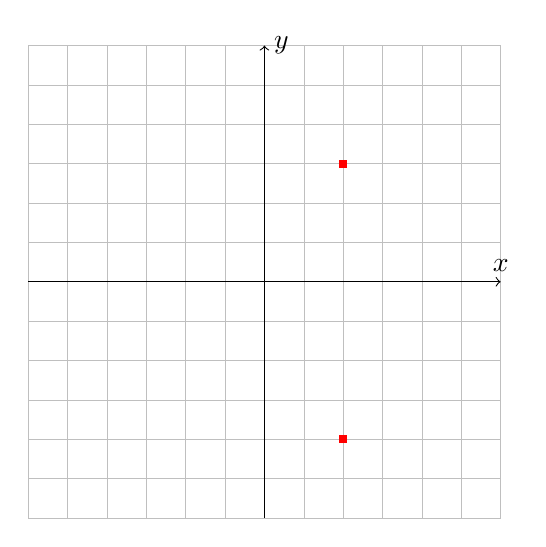
\begin{tikzpicture}[scale=0.5]
          \draw[lightgray,very thin] (-6,-6) grid (6,6);
          \draw[->] (-6,0)--(6,0) node[above]{$x$};
          \draw[->] (0,-6)--(0,6) node[right]{$y$};
          \node[fill=red,inner sep=1.5pt] (A) at (2,3) {};
          \node[fill=red,inner sep=1.5pt] (B) at (2,-4) {};
        \end{tikzpicture}
        &
        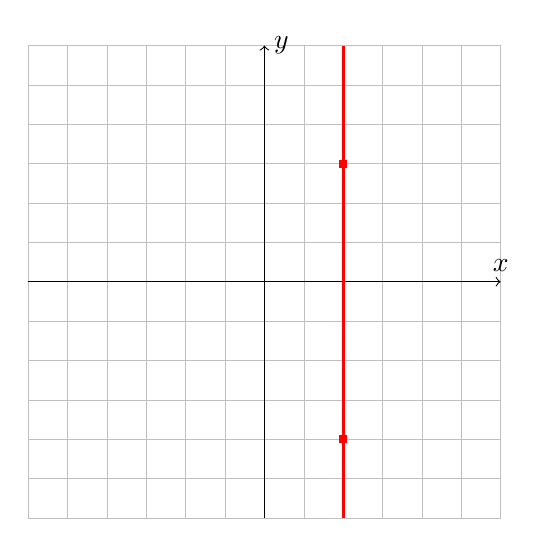
\begin{tikzpicture}[scale=0.5]
          \draw[lightgray,very thin] (-6,-6) grid (6,6);
          \draw[->] (-6,0)--(6,0) node[above]{$x$};
          \draw[->] (0,-6)--(0,6) node[right]{$y$};
          \draw[color=red,very thick] (2,-6)--(2,6);
          \node[fill=red,inner sep=1.5pt] (A) at (2,3) {};
          \node[fill=red,inner sep=1.5pt] (B) at (2,-4) {};
        \end{tikzpicture}
        \\
        \mbox{(a) Two points on the line}
        &
        \mbox{(b) Completed graph}
      \end{array}$
      \caption{Graph of $x=2$}
      \label{fig:x=2}
    \end{figure}
  \item % $\ds y=-3$
    This is similar to the previous problem.  Choose two points on the
    horizontal line $y=-3$, say $(-4,-3)$ and $(5,-3)$, then draw the
    line connecting them.  See Figure~\ref{fig:y=-3}.
    \begin{figure}[htbp]
      \centering
      $\begin{array}{c@{\hspace{1cm}}c}
        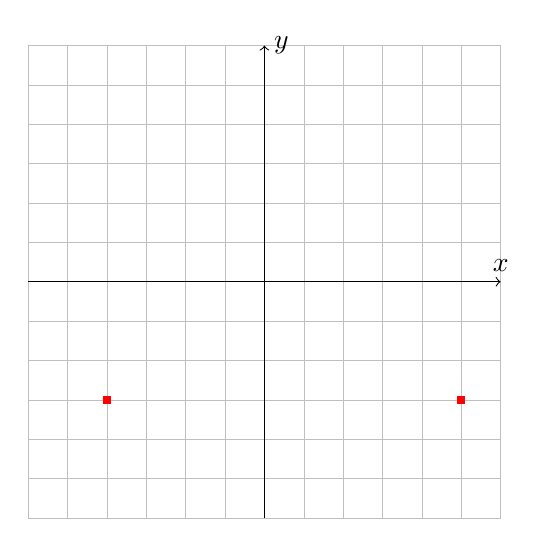
\begin{tikzpicture}[scale=0.5]
          \draw[lightgray,very thin] (-6,-6) grid (6,6);
          \draw[->] (-6,0)--(6,0) node[above]{$x$};
          \draw[->] (0,-6)--(0,6) node[right]{$y$};
          \node[fill=red,inner sep=1.5pt] (A) at (-4,-3) {};
          \node[fill=red,inner sep=1.5pt] (B) at (5,-3) {};
        \end{tikzpicture}
        &
        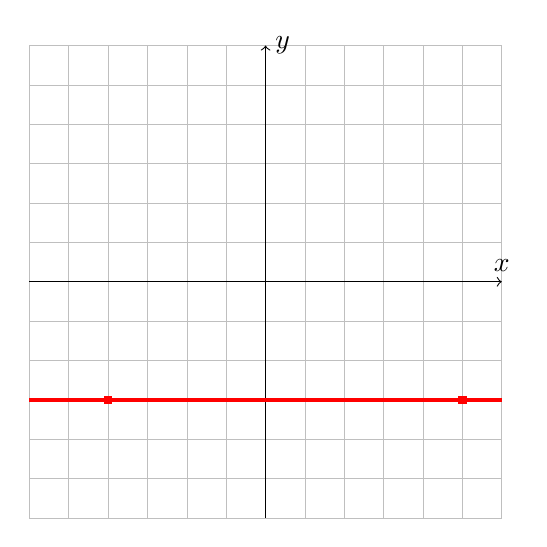
\begin{tikzpicture}[scale=0.5]
          \draw[lightgray,very thin] (-6,-6) grid (6,6);
          \draw[->] (-6,0)--(6,0) node[above]{$x$};
          \draw[->] (0,-6)--(0,6) node[right]{$y$};
          \draw[color=red,very thick] (-6,-3)--(6,-3);
          \node[fill=red,inner sep=1.5pt] (A) at (-4,-3) {};
          \node[fill=red,inner sep=1.5pt] (B) at (5,-3) {};
        \end{tikzpicture}
        \\
        \mbox{(a) Two points on the line}
        &
        \mbox{(b) Completed graph}
      \end{array}$
      \caption{Graph of $y=-3$}
      \label{fig:y=-3}
    \end{figure}
  \end{enumerate}
\item % (Based on B.21--36) Find an equation of the line that satisfies the
  % given conditions.
  \begin{enumerate}
  \item % Through $(-3,1)$, slope $-5/3$
    Since we have a point and a slope, we use point-slope form:
    \begin{equation*}
      y-y_1 = m(x-x_1) \implies y-1 = -\frac{5}{3} (x-(-3))
      \implies y-1 = -\frac{5}{3} (x+3)
    \end{equation*}
    The final simplification is optional.
  \item % Through $(1,-3)$ and $(-4,-2)$
    There are several ways to handle this problem, but I recommend
    first finding the slope of the line between the points:
    \begin{equation*}
      m = \frac{-2-(-3)}{-4-1} = \frac{-2+3}{-4-1} = \frac{1}{-5} =
      -\frac{1}{5} 
    \end{equation*}
    Now using the point $P(1,-3)$ as our point and $m=-1/5$ as our
    slope, we can use point-slope form:
    \begin{equation*}
      y-y_1 = m(x-x_1) \implies y-(-3) = -\frac{1}{5}(x-1)
      \implies y+3 = -\frac{1}{5}(x-1)
    \end{equation*}
    The latter simplification is optional in this context.
  \item % Slope $2$, $y$-intercept $5$
    We use the slope-intercept form with $m=2$ and $b=5$:
    \begin{equation*}
      y= mx+b \implies y = 2x + 5
    \end{equation*}
    % EJD: diagrams below
  \item % $x$-intercept $4$, $y$-intercept $-3$
    If the $x$-intercept is $4$, that means the line passes through
    the point $P(4,0)$.  Similarly, if the $y$-intercept is $-3$, that
    means the line passes through the point $Q(0,-3)$.  Next we find
    the slope:
    \begin{equation*}
      m = \frac{-3-0}{0-4} = \frac{-3}{-4} = \frac{3}{4}
    \end{equation*}
    Now we can use the point-slope form:
    \begin{equation*}
      y-y_1 = m(x-x_1) \implies y-0 = \frac{3}{4} (x-4)
      \implies y = \frac{3}{4} (x-4)
    \end{equation*}
  \item % Through $(1,-4)$, parallel to the $x$-axis
    You could use point-slope form, recalling that any line parallel
    to the $x$-axis has slope $0$:
    \begin{equation*}
      y-y_1 = m(x-x_1) \implies y-(-4) = 0 (x-1)
      \implies y+4 = 0 \implies y = -4
    \end{equation*}
    Either of the last two equations is acceptable as an answer.
  \item % Through $(1,-4)$, parallel to the $y$-axis
    The best way to answer this question is just to remember that all
    lines parallel to the $y$-axis have equation of the form $x=a$.
    Since the line passes through the point $(x,y)=(1,-4)$, we must
    have $a=1$.  So the equation of the line is $x=1$.
  \item % Through $(2,-3)$, parallel to the line $4x-5y=7$
    The slope of the given line can be found by putting it into
    slope-intercept form (solving for $y$).  We have
    \begin{equation*}
      4x-5y=7 \implies 5y = 4x-7 \implies y = \frac{4}{5} x -
      \frac{7}{5}
    \end{equation*}
    It follows that the slope of the given line is $4/5$.  Since
    parallel lines have the same slope, it follows that the slope of
    the unknown line is also $4/5$.  Now we have a point on the
    unknown line, $P(2,-3)$, and its slope, $m=4/5$, so we can use 
    point-slope form to write an equation for the line:
    \begin{equation*}
      y-y_1 = m(x-x_1) \implies y-(-3) = \frac{4}{5} (x-2)
      \implies y+3 = \frac{4}{5} (x-2)
    \end{equation*}
    where the latter simplification is optional.
  \item % Through $(-1/2,5/3)$, perpendicular to the line $3x+7y=2$
    Again, we first find the slope of the given line by solving for
    $y$:
    \begin{equation*}
      3x+7y=2 \implies 7y = -3x + 2 \implies y = -\frac{3}{7} x +
      \frac{2}{7}
    \end{equation*}
    so the slope of the given line is $-3/7$.  The slope of any
    perpendicular line is the negative reciprocal of that number so we
    can calculate
    \begin{equation*}
      m = -\frac{1}{-3/7} = -1 \times -\frac{7}{3} = \frac{7}{3}
    \end{equation*}
    (The end result can be obtained quickly by changing the sign
    (negative) and flipping the fraction over (reciprocal).)  Now we
    have a point on the unknown line, $P(-1/2,5/3)$, and its slope,
    $7/3$, so we can write an equation for the line in point-slope
    form:
    \begin{equation*}
      y-y_1 = m(x-x_1) 
      \implies 
      y-\frac{5}{3} = \frac{7}{3}\left(x-\left(-\frac{1}{2}\right)\right) 
      \implies y-\frac{5}{3} = \frac{7}{3}\left(x+\frac{1}{2}\right)
    \end{equation*}
    where the latter simplification is optional.  (Other optional
    simplifications may be helpful: you may find it easier to work
    with such an equation, for example, if you ``clear fractions'' by
    multiplying every term by $6$.)
  \end{enumerate}
\item % (Based on B.37--42) Find the slope and $y$-intercept of the line
  % and draw its graph.
  \begin{enumerate}
  \item % $\ds x+2y=0$ % EJD: maybe having 0 in here first is harder?
    To find the slope and $y$-intercept, we put the equation of the
    line into slope-intercept form by solving for $y$:
    \begin{equation*}
      x+2y=0 \implies y = -\frac{1}{2} x + 0
    \end{equation*}
    so the slope is $m=-1/2$ and the $y$-intercept is $(0,b)=(0,0)$.
    A second point could be found by substituting (say) $x=2$ into the
    equation of the line to obtain $y=(-1/2)(2)+0 = -1$ so $(2,-1)$ is
    a point on the line.  Plot the points $(0,0)$ and $(2,-1)$ and
    draw a line through them.  See~Figure{fig:x+2y=0}.
    \begin{figure}[htbp]
      \centering
      $\begin{array}{c@{\hspace{1cm}}c}
        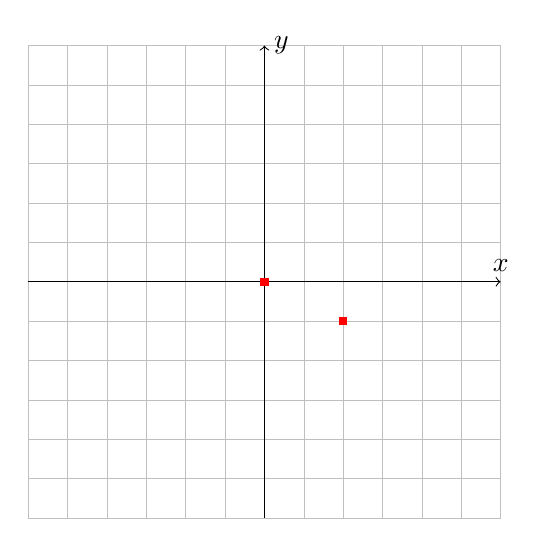
\begin{tikzpicture}[scale=0.5]
          \draw[lightgray,very thin] (-6,-6) grid (6,6);
          \draw[->] (-6,0)--(6,0) node[above]{$x$};
          \draw[->] (0,-6)--(0,6) node[right]{$y$};
          \node[fill=red,inner sep=1.5pt] (A) at (0,0) {};
          \node[fill=red,inner sep=1.5pt] (B) at (2,-1) {};
        \end{tikzpicture}
        &
        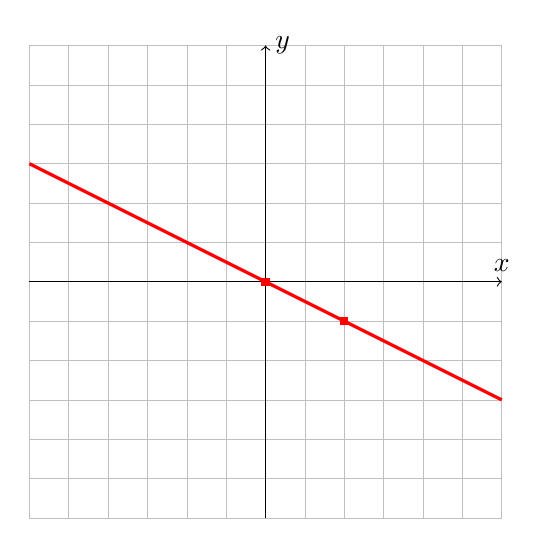
\begin{tikzpicture}[scale=0.5]
          \draw[lightgray,very thin] (-6,-6) grid (6,6);
          \draw[->] (-6,0)--(6,0) node[above]{$x$};
          \draw[->] (0,-6)--(0,6) node[right]{$y$};
          \draw[red,very thick] (-6,3)--(6,-3);
          \node[fill=red,inner sep=1.5pt] (A) at (0,0) {};
          \node[fill=red,inner sep=1.5pt] (B) at (2,-1) {};
        \end{tikzpicture}
        \\
        \mbox{(a) Two points on the line}
        &
        \mbox{(b) Completed graph}
      \end{array}$
      \caption{Graph of $x+2y=0$}
      \label{fig:x+2y=0}
    \end{figure}
  \item % $\ds 3x-4y=0$
    Putting the equation into slope-intercept form we have
    \begin{equation*}
      3x-4y=0 \implies 4y = 3x \implies y = \frac{3}{4} x + 0
    \end{equation*}
    so the slope is $m=3/4$ and the $y$-intercept is $(0,0)$.  We need
    a second point on the graph to determine the line.  We could solve
    as we solved the previous, or we could reason like this: since the
    slope is $3/4$, there is a rise of $3$ units for every run of $4$
    units.  Starting at $(0,0)$, we rise by $3$ and run by $4$ to get
    to $(4,3)$, which is therefore a second point on the graph.  We
    plot those to points and draw a line through them.  See
    Figure~\ref{fig:3x-4y=0}.
    \begin{figure}[htbp]
      \centering
      $\begin{array}{c@{\hspace{1cm}}c}
        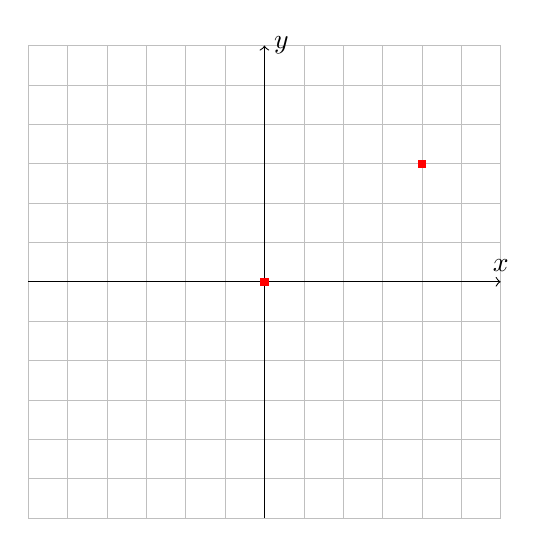
\begin{tikzpicture}[scale=0.5]
          \draw[lightgray,very thin] (-6,-6) grid (6,6);
          \draw[->] (-6,0)--(6,0) node[above]{$x$};
          \draw[->] (0,-6)--(0,6) node[right]{$y$};
          \node[fill=red,inner sep=1.5pt] (A) at (0,0) {};
          \node[fill=red,inner sep=1.5pt] (B) at (4,3) {};
        \end{tikzpicture}
        &
        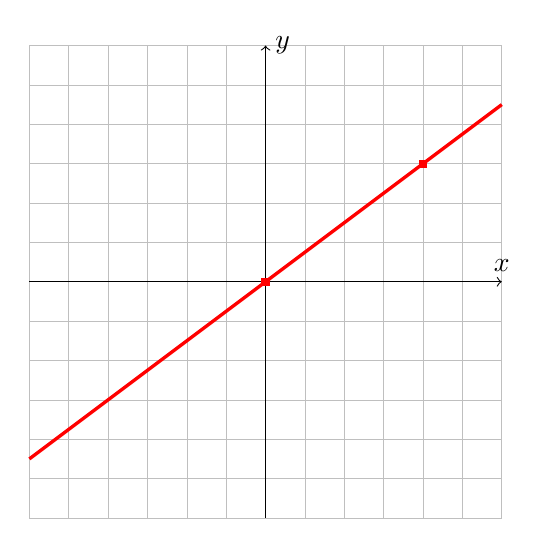
\begin{tikzpicture}[scale=0.5]
          \draw[lightgray,very thin] (-6,-6) grid (6,6);
          \draw[->] (-6,0)--(6,0) node[above]{$x$};
          \draw[->] (0,-6)--(0,6) node[right]{$y$};
          \draw[color=red,very thick] (-6,-4.5)--(6,4.5);
          \node[fill=red,inner sep=1.5pt] (A) at (0,0) {};
          \node[fill=red,inner sep=1.5pt] (B) at (4,3) {};
        \end{tikzpicture}
        \\
        \mbox{(a) Two points on the line}
        &
        \mbox{(b) Completed graph}
      \end{array}$
      \caption{Graph of $3x-4y=0$}
      \label{fig:3x-4y=0}
    \end{figure}
  \item % $\ds y=2$
    Writing in slope-intercept form, we have
    \begin{equation*}
      y=2 \implies y=0x + 2
    \end{equation*}
    so its slope is $0$ and $y$-intercept is $(0,2)$.  This is a line
    in horizontal form, so it's easy to graph on grid paper (it is the
    grid line parallel to the $x$-axis and passing through $(0,2)$).
    Or you could pick any two points of the form $(x,2)$, e.g.,
    $(-4,2)$, $(3,2)$, and draw the line through them.  See
    Figure~\ref{fig:y=2}. 
    \begin{figure}[htbp]
      \centering
      $\begin{array}{c@{\hspace{1cm}}c}
        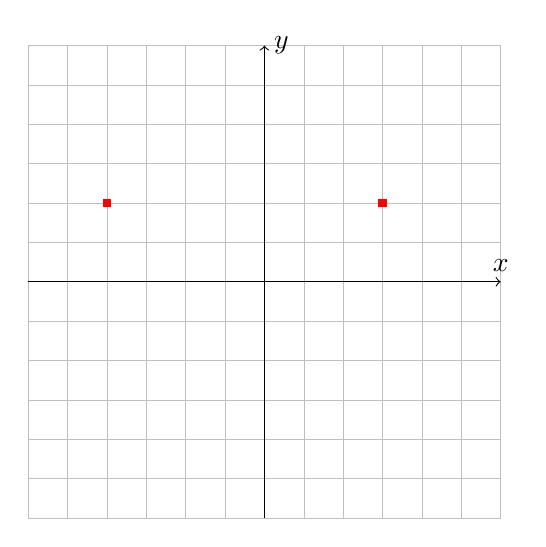
\begin{tikzpicture}[scale=0.5]
          \draw[lightgray,very thin] (-6,-6) grid (6,6);
          \draw[->] (-6,0)--(6,0) node[above]{$x$};
          \draw[->] (0,-6)--(0,6) node[right]{$y$};
          \node[fill=red,inner sep=1.5pt] (A) at (-4,2) {};
          \node[fill=red,inner sep=1.5pt] (B) at (3,2) {};
        \end{tikzpicture}
        &
        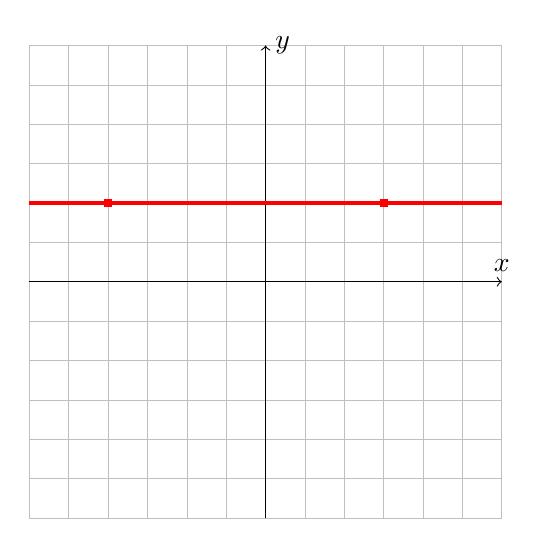
\begin{tikzpicture}[scale=0.5]
          \draw[lightgray,very thin] (-6,-6) grid (6,6);
          \draw[->] (-6,0)--(6,0) node[above]{$x$};
          \draw[->] (0,-6)--(0,6) node[right]{$y$};
          \draw[color=red,very thick] (-6,2)--(6,2);
          \node[fill=red,inner sep=1.5pt] (A) at (-4,2) {};
          \node[fill=red,inner sep=1.5pt] (B) at (3,2) {};
        \end{tikzpicture}
        \\
        \mbox{(a) Two points on the line}
        &
        \mbox{(b) Completed graph}
      \end{array}$
      \caption{Graph of $y=2$}
      \label{fig:y=2}
    \end{figure}
  \item\label{prob:3x-2y-5=0} % $\ds 3x-2y-5=0$
    The equation is given in general form.  Writing in slope-intercept
    form by solving for $y$,
    \begin{equation*}
      3x-2y-5=0 \implies 2y = 3x-5 \implies y = \frac{3}{2} x -
      \frac{5}{2}
    \end{equation*}
    so the slope is $m=3/2$ and the $y$-intercept is $(0,b)=(0,-5/2)$.
    We can find a second point on the line by substituting $x=3$ (say)
    to obtain $y=(3/2)(3) - (5/2) = 9/2 - 5/2 = 4/2 = 2$, so $(3,2)$
    is a second point on the line.  We plot those points and draw the
    line through them.  See Figure~\ref{fig:3x-2y-5=0}
    \begin{figure}[htbp]
      \centering
      $\begin{array}{c@{\hspace{1cm}}c}
        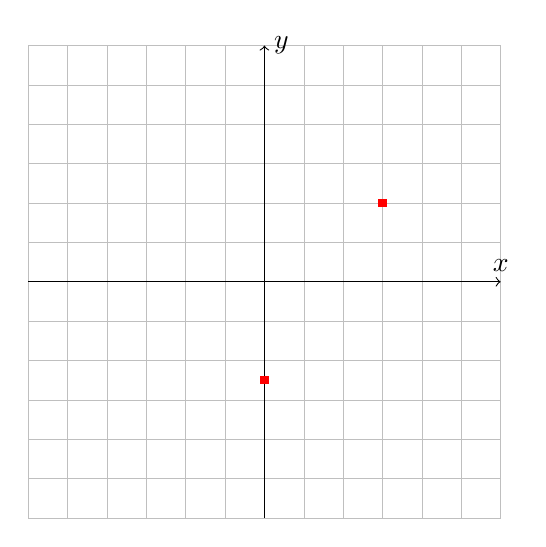
\begin{tikzpicture}[scale=0.5]
          \draw[lightgray,very thin] (-6,-6) grid (6,6);
          \draw[->] (-6,0)--(6,0) node[above]{$x$};
          \draw[->] (0,-6)--(0,6) node[right]{$y$};
          \node[fill=red,inner sep=1.5pt] (A) at (0,-2.5) {};
          \node[fill=red,inner sep=1.5pt] (B) at (3,2) {};
        \end{tikzpicture}
        &
        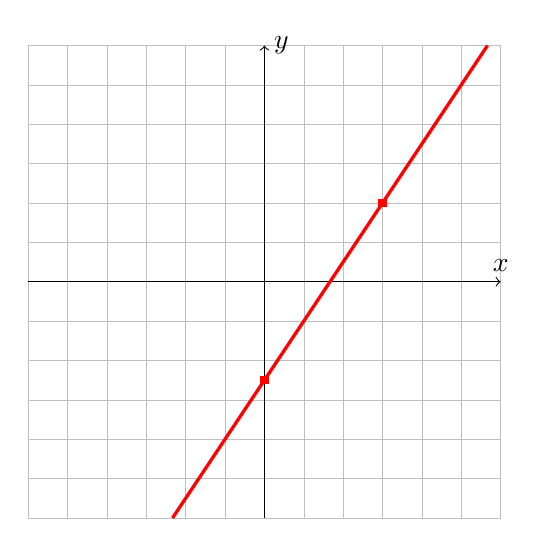
\begin{tikzpicture}[scale=0.5]
          \draw[lightgray,very thin] (-6,-6) grid (6,6);
          \draw[->] (-6,0)--(6,0) node[above]{$x$};
          \draw[->] (0,-6)--(0,6) node[right]{$y$};
          \draw[color=red,very thick] (-7/3,-6)--(17/3,6);
          \node[fill=red,inner sep=1.5pt] (A) at (0,-2.5) {};
          \node[fill=red,inner sep=1.5pt] (B) at (3,2) {};
        \end{tikzpicture}
        \\
        \mbox{(a) Two points on the line}
        &
        \mbox{(b) Completed graph}
      \end{array}$
      \caption{Graph of $3x-2y-5=0$}
      \label{fig:3x-2y-5=0}
    \end{figure}
  \end{enumerate}
\item\label{prob:graphineq} % (Based on B.43--49) 
  % Sketch the graph of the region in the $xy$-plane.
  \begin{enumerate}
  \item % $\ds \{(x,y)| y<0\}$
    We graph the line $y=0$ with a dashed line (because the
    intequality is strict, i.e., $y<0$ not $y\le 0$) and since $y$ is
    less than the expression that defines the line we shade all the
    points below the line.  See Figure~\ref{fig:yLT0}.
    \begin{figure}[htbp]
      \centering
      $\begin{array}{c@{\hspace{1cm}}c}
        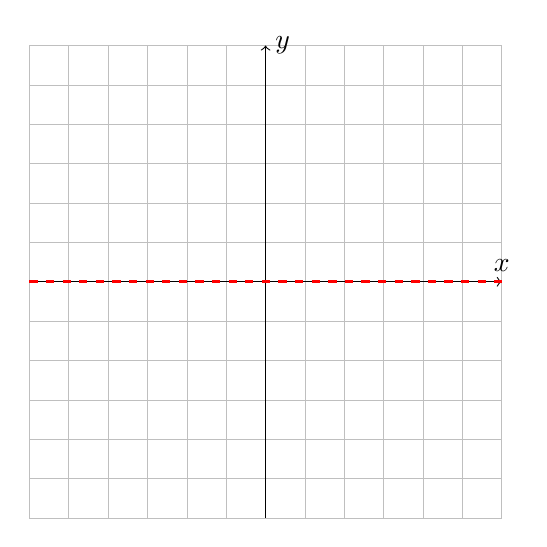
\begin{tikzpicture}[scale=0.5]
          \draw[lightgray,very thin] (-6,-6) grid (6,6);
          \draw[->] (-6,0)--(6,0) node[above]{$x$};
          \draw[->] (0,-6)--(0,6) node[right]{$y$};
          % EJD: better dashes; maybe don't draw x-axis
          \draw[color=red,very thick,dashed] (-6,0)--(6,0);
        \end{tikzpicture}
        &
        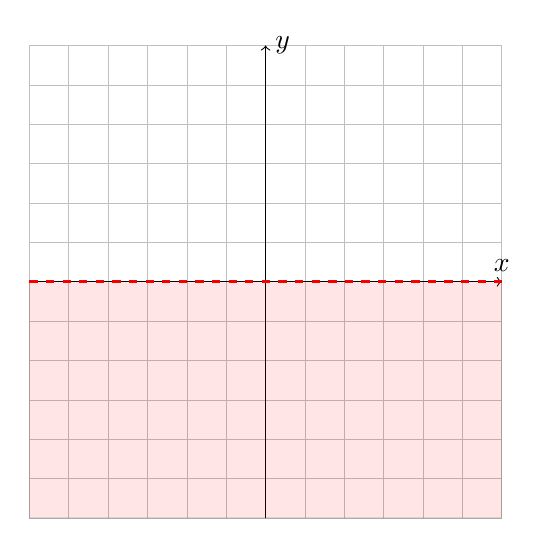
\begin{tikzpicture}[scale=0.5]
          \draw[lightgray,very thin] (-6,-6) grid (6,6);
          \draw[->] (-6,0)--(6,0) node[above]{$x$};
          \draw[->] (0,-6)--(0,6) node[right]{$y$};
          \draw[color=red,very thick,dashed] (-6,0)--(6,0);
          \draw[fill=red,very nearly transparent] %
          (-6,0)--(-6,-6)--(6,-6)--(6,0)--cycle; 
        \end{tikzpicture}
        \\
        \mbox{(a) Boundary $y=0$ of the region}
        &
        \mbox{(b) Completed graph}
      \end{array}$
      \caption{Graph of $y<0$}
      \label{fig:yLT0}
    \end{figure}
  \item % $\ds \{(x,y)| \mbox{$x\le 2$ and $y>1$}\}$ % EJD: this is not
                                % covered in the lecture!! $x\le 2$
    First we graph the vertical line $x=2$ with a solid line.  Then we
    shade all points to the left of the line, which gives us $x\le 2$.
    Then we graph the horizontal line $y=1$ with a dashed line.  Then
    we shade all points to the abve the line, which gives us $y>1$.
    All points which are ``double shaded'' are part of the final
    answer.  Note that the corner $(2,1)$ is not part of the final
    answer (why not?), so we draw it with an open circle for emphasis.
    See Figure~\ref{fig:xLE2andyGT1}.
    \begin{figure}[htbp]
      \centering
      $\begin{array}{c@{\hspace{1cm}}c}
        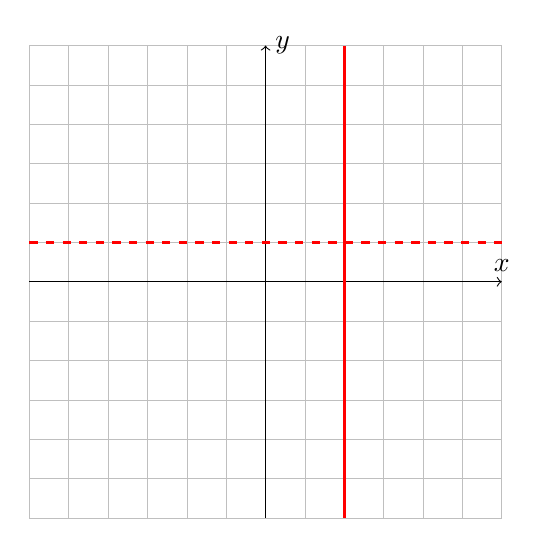
\begin{tikzpicture}[scale=0.5]
          \draw[lightgray,very thin] (-6,-6) grid (6,6);
          \draw[->] (-6,0)--(6,0) node[above]{$x$};
          \draw[->] (0,-6)--(0,6) node[right]{$y$};
          \draw[color=red,very thick] (2,-6)--(2,6);
          % EJD: better dashes
          \draw[color=red,very thick,dashed] (-6,1)--(6,1);
        \end{tikzpicture}
        &
        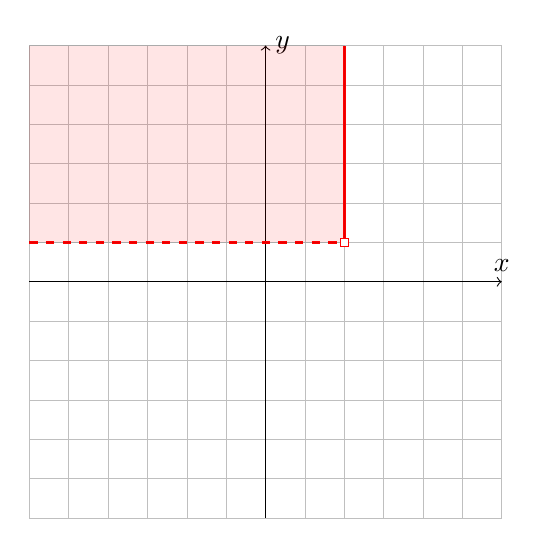
\begin{tikzpicture}[scale=0.5]
          \draw[lightgray,very thin] (-6,-6) grid (6,6);
          \draw[->] (-6,0)--(6,0) node[above]{$x$};
          \draw[->] (0,-6)--(0,6) node[right]{$y$};
          \draw[color=red,very thick] (2,1)--(2,6);
          % EJD: better dashes
          \draw[color=red,very thick,dashed] (-6,1)--(2,1);
          \draw[fill=red,very nearly transparent] %
          (-6,1)--(2,1)--(2,6)--(-6,6)--cycle;
          \node[draw=red,fill=white,inner sep=1.5pt] (A) at (2,1) {};
        \end{tikzpicture}
        \\
        \mbox{(a) Boundary of the region}
        &
        \mbox{(b) Completed graph}
      \end{array}$
      \caption{Graph of $x\le 2$ and $y>1$}
      \label{fig:xLE2andyGT1}
    \end{figure}
  \item % $\ds \{(x,y)| |y|<3\}$
    The condition without absolute values translates to ``$-3<y$ and
    $y<3$''.  We graph each of those regions by the method of the
    previous problems and combine them to obtain the final result. 
    See Figure~\ref{fig:absyLT3}.
    \begin{figure}[htbp]
      \centering
      $\begin{array}{c@{\hspace{1cm}}c}
        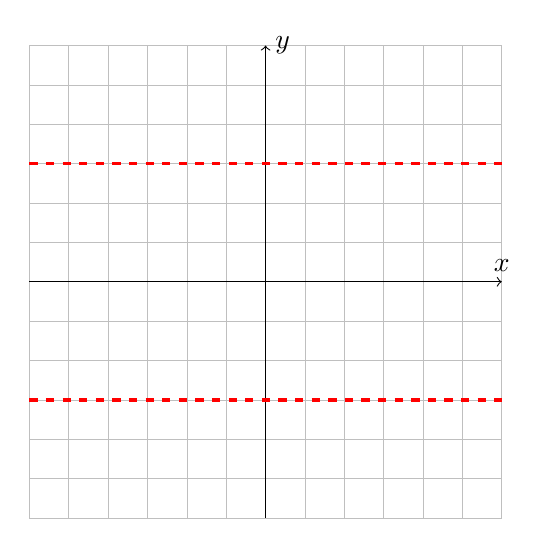
\begin{tikzpicture}[scale=0.5]
          \draw[lightgray,very thin] (-6,-6) grid (6,6);
          \draw[->] (-6,0)--(6,0) node[above]{$x$};
          \draw[->] (0,-6)--(0,6) node[right]{$y$};
          \draw[color=red,very thick, dashed] (-6,-3)--(6,-3);
          \draw[color=red,very thick, dashed] (-6,3)--(6,3);
        \end{tikzpicture}
        &
        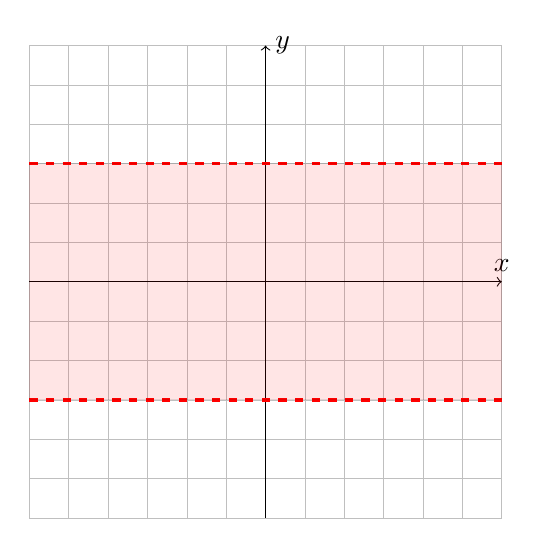
\begin{tikzpicture}[scale=0.5]
          \draw[lightgray,very thin] (-6,-6) grid (6,6);
          \draw[->] (-6,0)--(6,0) node[above]{$x$};
          \draw[->] (0,-6)--(0,6) node[right]{$y$};
          \draw[color=red,very thick, dashed] (-6,-3)--(6,-3);
          \draw[color=red,very thick, dashed] (-6,3)--(6,3);
          \draw[fill=red,very nearly transparent] %
          (-6,3)--(6,3)--(6,-3)--(-6,-3)--cycle;
        \end{tikzpicture}
        \\
        \mbox{(a) Boundary of the region}
        &
        \mbox{(b) Completed graph}
      \end{array}$
      \caption{Graph of $|y|<3$}
      \label{fig:absyLT3}
    \end{figure}
  \item % $\ds \{(x,y)| \mbox{$\|x\|<4$ and $\|y\|<3$}\}$
    The first condition translates to ``$-4<x$ and $x<4$'', while the
    second condition translates to ``$-3<y$ and $y<3$''.  We graph
    each of those regions, and the answer is the resulting ``quadruple-shaded''
    region, also known as an ``open box'' (\textit{open} because it does not
    include its boundary).
    \begin{figure}[htbp]
      \centering
      $\begin{array}{c@{\hspace{1cm}}c}
        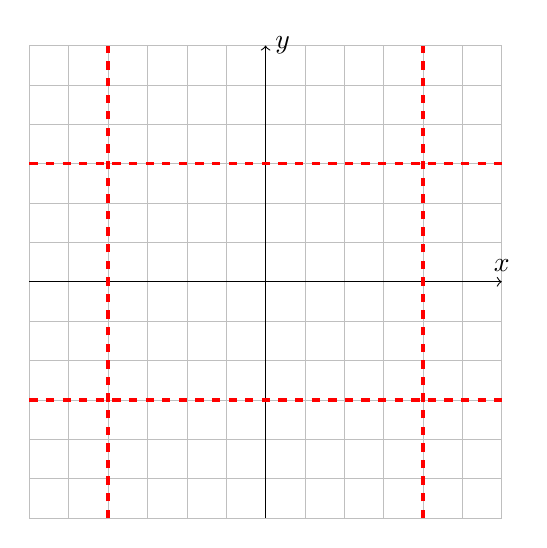
\begin{tikzpicture}[scale=0.5]
          \draw[lightgray,very thin] (-6,-6) grid (6,6);
          \draw[->] (-6,0)--(6,0) node[above]{$x$};
          \draw[->] (0,-6)--(0,6) node[right]{$y$};
          \draw[color=red,very thick,dashed] (4,-6)--(4,6);
          \draw[color=red,very thick,dashed] (-4,-6)--(-4,6);
          \draw[color=red,very thick,dashed] (-6,3)--(6,3);
          \draw[color=red,very thick,dashed] (-6,-3)--(6,-3);
        \end{tikzpicture}
        &
        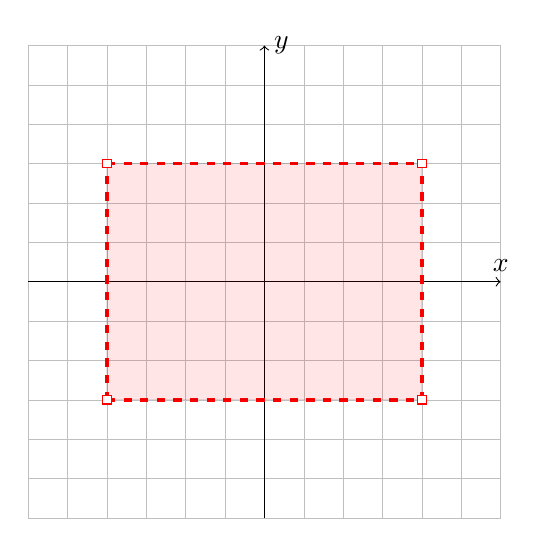
\begin{tikzpicture}[scale=0.5]
          \draw[lightgray,very thin] (-6,-6) grid (6,6);
          \draw[->] (-6,0)--(6,0) node[above]{$x$};
          \draw[->] (0,-6)--(0,6) node[right]{$y$};
          \draw[color=red,very thick,dashed] (4,-3)--(4,3);
          \draw[color=red,very thick,dashed] (-4,-3)--(-4,3);
          \draw[color=red,very thick,dashed] (-4,3)--(4,3);
          \draw[color=red,very thick,dashed] (-4,-3)--(4,-3);
          \draw[fill=red,very nearly transparent] %
          (-4,-3)--(4,-3)--(4,3)--(-4,3)--cycle; 
          \node[draw=red,fill=white,inner sep=1.5pt] (A) at (-4,-3) {};
          \node[draw=red,fill=white,inner sep=1.5pt] (A) at (4,-3) {};
          \node[draw=red,fill=white,inner sep=1.5pt] (A) at (4,3) {};
          \node[draw=red,fill=white,inner sep=1.5pt] (A) at (-4,3) {};
        \end{tikzpicture}
        \\
        \mbox{(a) Boundary of the region}
        &
        \mbox{(b) Completed graph}
      \end{array}$
      \caption{Graph of $|x|<4$ and $|y|<3$}
      \label{fig:absxLT4andabsyLT3}
    \end{figure}
  \end{enumerate}
\item % (Based on B.11) Consider the points $A(1,0)$, 
  % $B(-2,-3)$, and $C(-3,1)$.
  % Show that the distance between $A$ and $C$ is the same as the distance
  % between $B$ and $C$.
  The distances are the same because
  \begin{align*}
    |AC| &= \sqrt{(-3-1)^2 + (1-0)^2} = \sqrt{16+1} = \sqrt{17} \\
    |BC| &= \sqrt{(-3-(-2))^2 + (1-(-3))^2} = \sqrt{1+16} = \sqrt{17}
  \end{align*}
\item % (Based on B.14) 
  \begin{enumerate}
  \item % Show that the points $A(-4,7)$, $B(0,-5)$, and $C(2,-11)$ are
    % collinear (lie on the same line) by showing that
    % $|AB|+|BC|=|AC|$.
    % EJD: is the Stewart version of the problem this hard?
    We have
    \begin{align*}
      |AB| 
      &= \sqrt{(0-(-4))^2 + (-5-7)^2} = \sqrt{16+144} = \sqrt{160} =
        \sqrt{16} \, \sqrt{10} = 4\sqrt{10}
      \\
      |BC| 
      &= \sqrt{(2-0)^2+(-11-(-5))^2} = \sqrt{4+36} = \sqrt{40} =
      \sqrt{4} \, \sqrt{10} = 2\sqrt{10}
      \\
      |AC| 
      &= \sqrt{(2-(-4))^2 + (-11-7)^2} = \sqrt{36+324} =
      \sqrt{360} = \sqrt{36} \, \sqrt{10} = 6\sqrt{10}
    \end{align*}
    So we see that $|AB| + |BC| = 4\sqrt{10} + 2\sqrt{10} = 6\sqrt{10}
    = |AC|$.  If $B$ were not directly between $A$ and $C$, the trip
    from $A$ through $B$ to $C$ would be longer than the trip
    directly from $A$ to $C$.  % EJD: diagrams
  \item Use slopes to show that $A$, $B$, and $C$ are collinear.
    The slopes of the lines are
    \begin{align*}
      \operatorname{slope}(AB) 
      &= \frac{-5-7}{0-(-4)} = \frac{-12}{4} = -3 \\
      \operatorname{slope}(BC)
      &= \frac{-11-(-5)}{2-0} = \frac{-6}{2} = -3 
    \end{align*}
    If $B$ did not lie on the line betwen $A$ and $C$, there would be
    a ``kink'' on the path from $A$ to $B$ to $C$ and the slopes would
    be different.  Since the slopes are the same, $B$ does lie on the
    line from $A$ to $C$.
  \end{enumerate}
\item % (Based on B.19--20) Sketch the graph of the equation.
  % EJD: this is straightforward, not hard -- reorder
  \begin{enumerate}
  \item % $\ds |x|=2$
    This is similar to question~\ref{prob:graphineq}.  The condition
    translates to ``$x=-2$ or $x=2$'', so we graph those two vertical
    lines.  See Figure~\ref{fig:absx=2ANDxy=0}(a).
    \begin{figure}[htbp]
      \centering
      $\begin{array}{c@{\hspace{1cm}}c}
        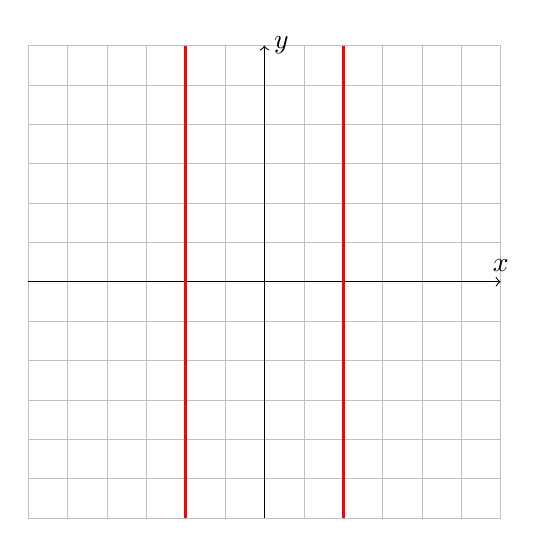
\begin{tikzpicture}[scale=0.5]
          \draw[lightgray,very thin] (-6,-6) grid (6,6);
          \draw[->] (-6,0)--(6,0) node[above]{$x$};
          \draw[->] (0,-6)--(0,6) node[right]{$y$};
          \draw[color=red,very thick] (-2,-6)--(-2,6);
          \draw[color=red,very thick] (2,-6)--(2,6);
        \end{tikzpicture}
        &
        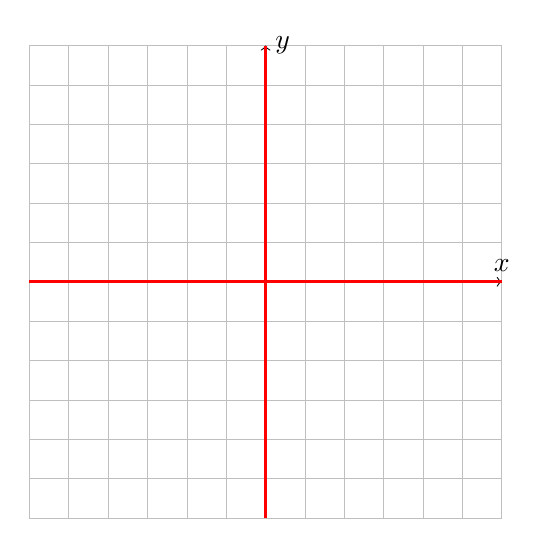
\begin{tikzpicture}[scale=0.5]
          \draw[lightgray,very thin] (-6,-6) grid (6,6);
          \draw[->] (-6,0)--(6,0) node[above]{$x$};
          \draw[->] (0,-6)--(0,6) node[right]{$y$};
          \draw[color=red,very thick] (-6,0)--(6,0);
          \draw[color=red,very thick] (0,-6)--(0,6);
        \end{tikzpicture}
        \\
        \mbox{(a) Graph of $|x|=2$}
        &
        \mbox{(b) Graph of $xy=0$}
      \end{array}$
      \caption{Two graphs}
      \label{fig:absx=2ANDxy=0}
    \end{figure}
  \item % $\ds xy=0$
    Factoring, the condition $xy=0$ reduces to ``$x=0$ or $y=0$''.
    The line $x=0$ is the $y$-axis, and the line $y=0$ is the
    $x$-axis.
    See Figure~\ref{fig:absx=2ANDxy=0}(b).
  \end{enumerate}
\item % (Based on B.50--52) Sketch the region in the $xy$-plane.
  \begin{enumerate}
  \item % $\ds \{(x,y) | 2y<3x-5\}$
    Solving for $y$, the condition is $y<(3/2)x-(5/2)$.  We graphed
    this line in question~\ref{prob:3x-2y-5=0}, so we can just re-draw the
    graph (but with a dotted line).  Then we shade the region below
    the line. 
    See Figure~\ref{fig:2yLT3x-5AND3-xLTyLT3+2x}(a).
    \begin{figure}[htbp]
      \centering
      $\begin{array}{c@{\hspace{1cm}}c}
        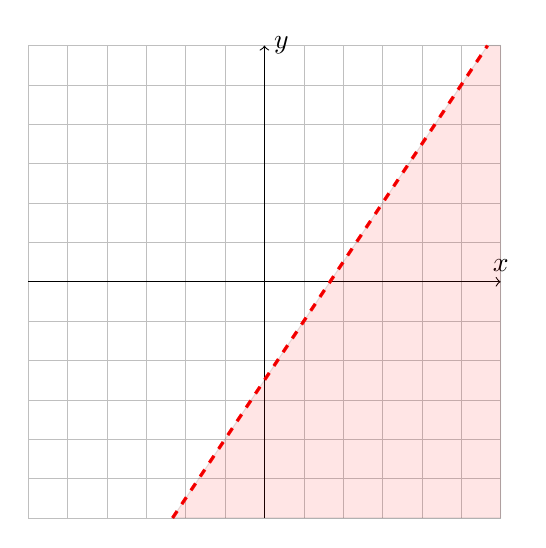
\begin{tikzpicture}[scale=0.5]
          \draw[lightgray,very thin] (-6,-6) grid (6,6);
          \draw[->] (-6,0)--(6,0) node[above]{$x$};
          \draw[->] (0,-6)--(0,6) node[right]{$y$};
          \draw[color=red,very thick,dashed] (-7/3,-6)--(17/3,6);
          \draw[fill=red,very nearly transparent]
          (-7/3,-6)--(17/3,6)--(6,6)--(6,-6)--cycle; 
        \end{tikzpicture}
        &
        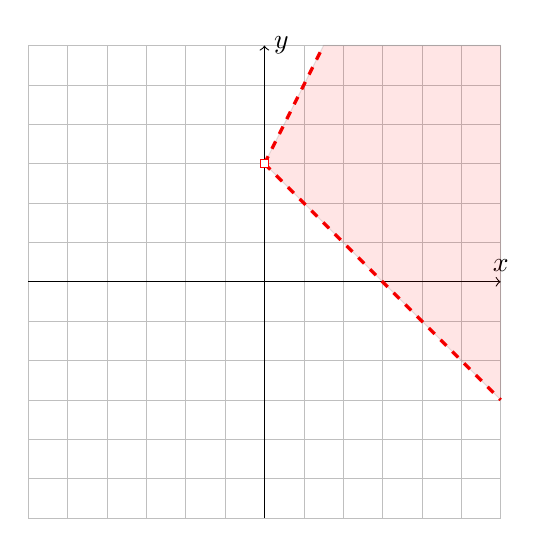
\begin{tikzpicture}[scale=0.5]
          \draw[lightgray,very thin] (-6,-6) grid (6,6);
          \draw[->] (-6,0)--(6,0) node[above]{$x$};
          \draw[->] (0,-6)--(0,6) node[right]{$y$};
          \draw[color=red,very thick,dashed] (0,3)--(6,-3);
          \draw[color=red,very thick,dashed] (0,3)--(3/2,6);
          \draw[fill=red,very nearly transparent] %
          (0,3)--(3/2,6)--(6,6)--(6,-3)--cycle; 
          \node[draw=red,fill=white,inner sep=1.5pt] (A) at (0,3) {};
        \end{tikzpicture}
        \\
        \mbox{Graph of $2y<3x-5$}
        &
        \mbox{Graph of $3-x<y<3+2x$}
      \end{array}$
      \caption{Two graphs}
      \label{fig:2yLT3x-5AND3-xLTyLT3+2x}
    \end{figure}
  \item % $\ds \{(x,y) | 3-x<y<3+2x\}$
    The two conditions are $y>3-x$ and $y<2x+3$.  We graph each of
    those lines with dashed lines, shade the region above the first
    and below the second, and the final result is the region that is
    double-shaded.  See Figure~\ref{fig:2yLT3x-5AND3-xLTyLT3+2x}(b).
    Note that I have also marked the intersection of the two lines,
    which has coordinate $(0,3)$.  (How can you find that intersection?)
  \end{enumerate}
\item % (Based on B.53) Find a point on the $y$-axis that is equidistant from
  % $(4,-3)$ and $(2,5)$.
  % EJD:diagram 
  Points on the $y$-axis are of the form $(0,y)$.  The distance from
  such a point to $(4,-3)$ is
  \begin{equation*}
    \sqrt{(-3-y)^2+(4-0)^2} = \sqrt{(y+3)^2 + 16} = \sqrt{y^2+6y+25}
  \end{equation*}
  The distance from such a point to $(2,5)$ is
  \begin{equation*}
    \sqrt{(5-y)^2+(2-0)^2} = \sqrt{y^2-10y+29}
  \end{equation*}
  If the point $(0,y)$ is equidistance from the two given points, we
  must have
  \begin{equation*}
    \sqrt{y^2+6y+25} = \sqrt{y^2-10y+29}
  \end{equation*}
  Squaring both sides, we get 
  \begin{equation*}
    y^2 + 6y + 25 = y^2 - 10y + 29
    \implies 16y = 4 
    \implies y = \frac{1}{4}
  \end{equation*}
  So the point $(0,1/4)$ satisfies the conditions of the problem.
  (Check!)
  
  If you are familiar with geometry, another (better) way to solve
  this problem would be to find the intersection of two lines, the
  $y$-axis and the perpendicular bisector of the segment connecting
  the two points.
\end{enumerate}
\end{document}

